\documentclass[a4paper,12pt]{article}
\usepackage[utf8]{inputenc}
\usepackage{amsmath}
\usepackage{amssymb}
\usepackage{graphicx}
\usepackage{geometry}
\usepackage{tikz}
\usepackage{pgfplots}
\pgfplotsset{width=9cm, compat=1.9}
\usepackage{multicol}
\usepackage{array}
\setlength{\columnsep}{1cm}
\usepackage[inline]{enumitem}
\usepackage{setspace}
\usepackage{subcaption}
\usepackage{array}
\newcolumntype{L}[1]{>{\raggedright\let\newline\\\arraybackslash\hspace{0pt}}m{#1}}
\newcolumntype{C}[1]{>{\centering\let\newline\\\arraybackslash\hspace{0pt}}m{#1}}
\newcolumntype{R}[1]{>{\raggedleft\let\newline\\\arraybackslash\hspace{0pt}}m{#1}}
\usepackage{tcolorbox}
\usepackage{listofitems}
\renewcommand{\arraystretch}{1.5}
\geometry{a4paper, margin=1.5cm}
\setlength\parindent{0pt}
\newcommand\boxes[7]{
\begin{tikzpicture}
\newcommand{\wid}{1.6cm}
\newcommand{\hgt}{1cm}
\newcommand{\brd}{0.4cm}
\draw[](0,0)rectangle(0+\wid,0+\hgt);
\draw[](\wid/2,\hgt/2)node[]{#1};
\draw[](0-\wid/2,0-\hgt)rectangle(0+\wid/2,0);
\draw[](0,-\hgt/2)node[]{#2};
\draw[](0+\wid/2,0-\hgt)rectangle(0+3*\wid/2,0);
\draw[](\wid,-\hgt/2)node[]{#3};
\draw[](0-\wid,0-2*\hgt)rectangle(0,-\hgt);
\draw[](-\wid/2,-3*\hgt/2)node[]{#4};
\draw[](0,0-2*\hgt)rectangle(\wid,-\hgt);
\draw[](\wid/2,-3*\hgt/2)node[]{#5};
\draw[](0+\wid,0-2*\hgt)rectangle(2*\wid,-\hgt);
\draw[](3*\wid/2,-3*\hgt/2)node[]{#6};
\draw[white](-\wid-\brd,-2*\hgt-\brd)rectangle(2*\wid+\brd,\hgt+\brd);
\draw[](-\wid-\brd,\hgt+\brd)node[anchor= north west]{\textbf{#7)}};

\end{tikzpicture}
}
\newcommand\boxesSols[7]{
	\begin{tikzpicture}[scale=0.75]
	\newcommand{\wid}{1.6cm}
	\newcommand{\hgt}{1cm}
	\newcommand{\brd}{0.4cm}
	\draw[](0,0)rectangle(0+\wid,0+\hgt);
	\draw[](\wid/2,\hgt/2)node[]{#1};
	\draw[](0-\wid/2,0-\hgt)rectangle(0+\wid/2,0);
	\draw[](0,-\hgt/2)node[]{#2};
	\draw[](0+\wid/2,0-\hgt)rectangle(0+3*\wid/2,0);
	\draw[](\wid,-\hgt/2)node[]{#3};
	\draw[](0-\wid,0-2*\hgt)rectangle(0,-\hgt);
	\draw[](-\wid/2,-3*\hgt/2)node[]{#4};
	\draw[](0,0-2*\hgt)rectangle(\wid,-\hgt);
	\draw[](\wid/2,-3*\hgt/2)node[]{#5};
	\draw[](0+\wid,0-2*\hgt)rectangle(2*\wid,-\hgt);
	\draw[](3*\wid/2,-3*\hgt/2)node[]{#6};
	\draw[white](-\wid-\brd,-2*\hgt-\brd)rectangle(2*\wid+\brd,\hgt+\brd);
	\draw[](-\wid-\brd,\hgt+\brd)node[anchor= north west]{\textbf{#7)}};
	
	\end{tikzpicture}
}
\newcommand\magicsquare[9]{
\begin{tikzpicture}
\newcommand{\wid}{1.5cm}
\newcommand{\hgt}{1.5cm}
\newcommand{\brd}{0.3cm}
\draw[](0,0)rectangle(3*\wid,3*\hgt);
\draw[pink](0-\brd,0-5*\brd)rectangle(3*\wid+5*\brd,3*\hgt+\brd);
\draw[](\wid,0)--(\wid,3*\hgt);
\draw[](2*\wid,0)--(2*\wid,3*\hgt);
\draw[](0,\hgt)--(3*\wid,\hgt);
\draw[](0,2*\hgt)--(3*\wid,2*\hgt);
\draw[](\wid/2,\hgt/2)node[]{\Large #1};
\draw[](\wid/2,3*\hgt/2)node[]{\Large #2};
\draw[](\wid/2,5*\hgt/2)node[]{\Large #3};
\draw[](3*\wid/2,\hgt/2)node[]{\Large #4};
\draw[](3*\wid/2,3*\hgt/2)node[]{\Large #5};
\draw[](3*\wid/2,5*\hgt/2)node[]{\Large #6};
\draw[](5*\wid/2,\hgt/2)node[]{\Large #7};
\draw[](5*\wid/2,3*\hgt/2)node[]{\Large #8};
\draw[](5*\wid/2,5*\hgt/2)node[]{\Large #9};
\draw(0,-0.75)node[right]{\Large \textbf{Magic Number =}};


\end{tikzpicture}	
}

%first 9 arguments are  numbers for the square: row by row, top down, left to right
%numbers are separated by commas
%the 10th number is the question number
\newcommand\magicsquareA[1]{
	\setsepchar{,}
	\readlist\arg{#1} 
	\begin{tikzpicture}
	\newcommand{\wid}{1.3cm}
	\newcommand{\hgt}{1.3cm}
	\newcommand{\brd}{0.5cm}
	\draw[](0,0)rectangle(3*\wid,3*\hgt);
	\draw[](0-\brd,3*\hgt+1.2*\brd)node[anchor=north west]{\textbf{\arg[10])}};
\draw[white](0-\brd,0-2*\brd)rectangle(3*\wid+3*\brd,3*\hgt+\brd);
	\draw[](\wid,0)--(\wid,3*\hgt);
	\draw[](2*\wid,0)--(2*\wid,3*\hgt);
	\draw[](0,\hgt)--(3*\wid,\hgt);
	\draw[](0,2*\hgt)--(3*\wid,2*\hgt);
	\draw[](\wid/2,\hgt/2)node[]{\Large \arg[7]};
	\draw[](\wid/2,3*\hgt/2)node[]{\Large \arg[4]};
	\draw[](\wid/2,5*\hgt/2)node[]{\Large \arg[1]};
	\draw[](3*\wid/2,\hgt/2)node[]{\Large \arg[8]};
	\draw[](3*\wid/2,3*\hgt/2)node[]{\Large \arg[5]};
	\draw[](3*\wid/2,5*\hgt/2)node[]{\Large \arg[2]};
	\draw[](5*\wid/2,\hgt/2)node[]{\Large \arg[9]};
	\draw[](5*\wid/2,3*\hgt/2)node[]{\Large \arg[6]};
	\draw[](5*\wid/2,5*\hgt/2)node[]{\Large \arg[3]};
	\draw(0,-0.75)node[right]{\footnotesize \textbf{Magic Number =$\arg[11]$}};
	\end{tikzpicture}	
}

\newcommand\magicsquareASols[1]{
	\setsepchar{,}
	\readlist\arg{#1} 
	\begin{tikzpicture}[scale=0.75]
	\newcommand{\wid}{1.3cm}
	\newcommand{\hgt}{1.3cm}
	\newcommand{\brd}{0.5cm}
	\draw[](0,0)rectangle(3*\wid,3*\hgt);
	\draw[](0-\brd,3*\hgt+1.2*\brd)node[anchor=north west]{\textbf{\arg[10])}};
	\draw[white](0-\brd,0-2*\brd)rectangle(3*\wid+3*\brd,3*\hgt+\brd);
	\draw[](\wid,0)--(\wid,3*\hgt);
	\draw[](2*\wid,0)--(2*\wid,3*\hgt);
	\draw[](0,\hgt)--(3*\wid,\hgt);
	\draw[](0,2*\hgt)--(3*\wid,2*\hgt);
	\draw[](\wid/2,\hgt/2)node[]{\Large \arg[7]};
	\draw[](\wid/2,3*\hgt/2)node[]{\Large \arg[4]};
	\draw[](\wid/2,5*\hgt/2)node[]{\Large \arg[1]};
	\draw[](3*\wid/2,\hgt/2)node[]{\Large \arg[8]};
	\draw[](3*\wid/2,3*\hgt/2)node[]{\Large \arg[5]};
	\draw[](3*\wid/2,5*\hgt/2)node[]{\Large \arg[2]};
	\draw[](5*\wid/2,\hgt/2)node[]{\Large \arg[9]};
	\draw[](5*\wid/2,3*\hgt/2)node[]{\Large \arg[6]};
	\draw[](5*\wid/2,5*\hgt/2)node[]{\Large \arg[3]};
	\draw(0,-0.75)node[right]{\footnotesize \textbf{Magic Number =$\arg[11]$}};
	\end{tikzpicture}	
}


\begin{document}
\thispagestyle{empty}	
	\Large
	\begin{figure} 
		\centering
		
\includegraphics[height=4cm]{Marsden_green_on_white.jpg}
		\caption*{February 2018}
	\end{figure}
	.
\vspace{3cm}
	\begin{center}
			\textbf{Year 9 Number 1 Booklet}
	\end{center}

	\vspace{3cm}
	
	\normalsize
	\newpage
	\tableofcontents
	\newpage
	
	\section{Prime Numbers}
	Prime Numbers: a prime number is a number that has no factors other than itself and 1.\\
	\textbf{The first prime number is 2}.\\\\
	On the grid below, leave 2 unshaded but shade out all multiples of 2 (i.e 4,6,8,…).\\ 
	Go to the next unshaded number and leave that unshaded but shade out all multiples of that number.
	Repeat the process until you have found all of the prime numbers less than 100.
	
	\begin{center}
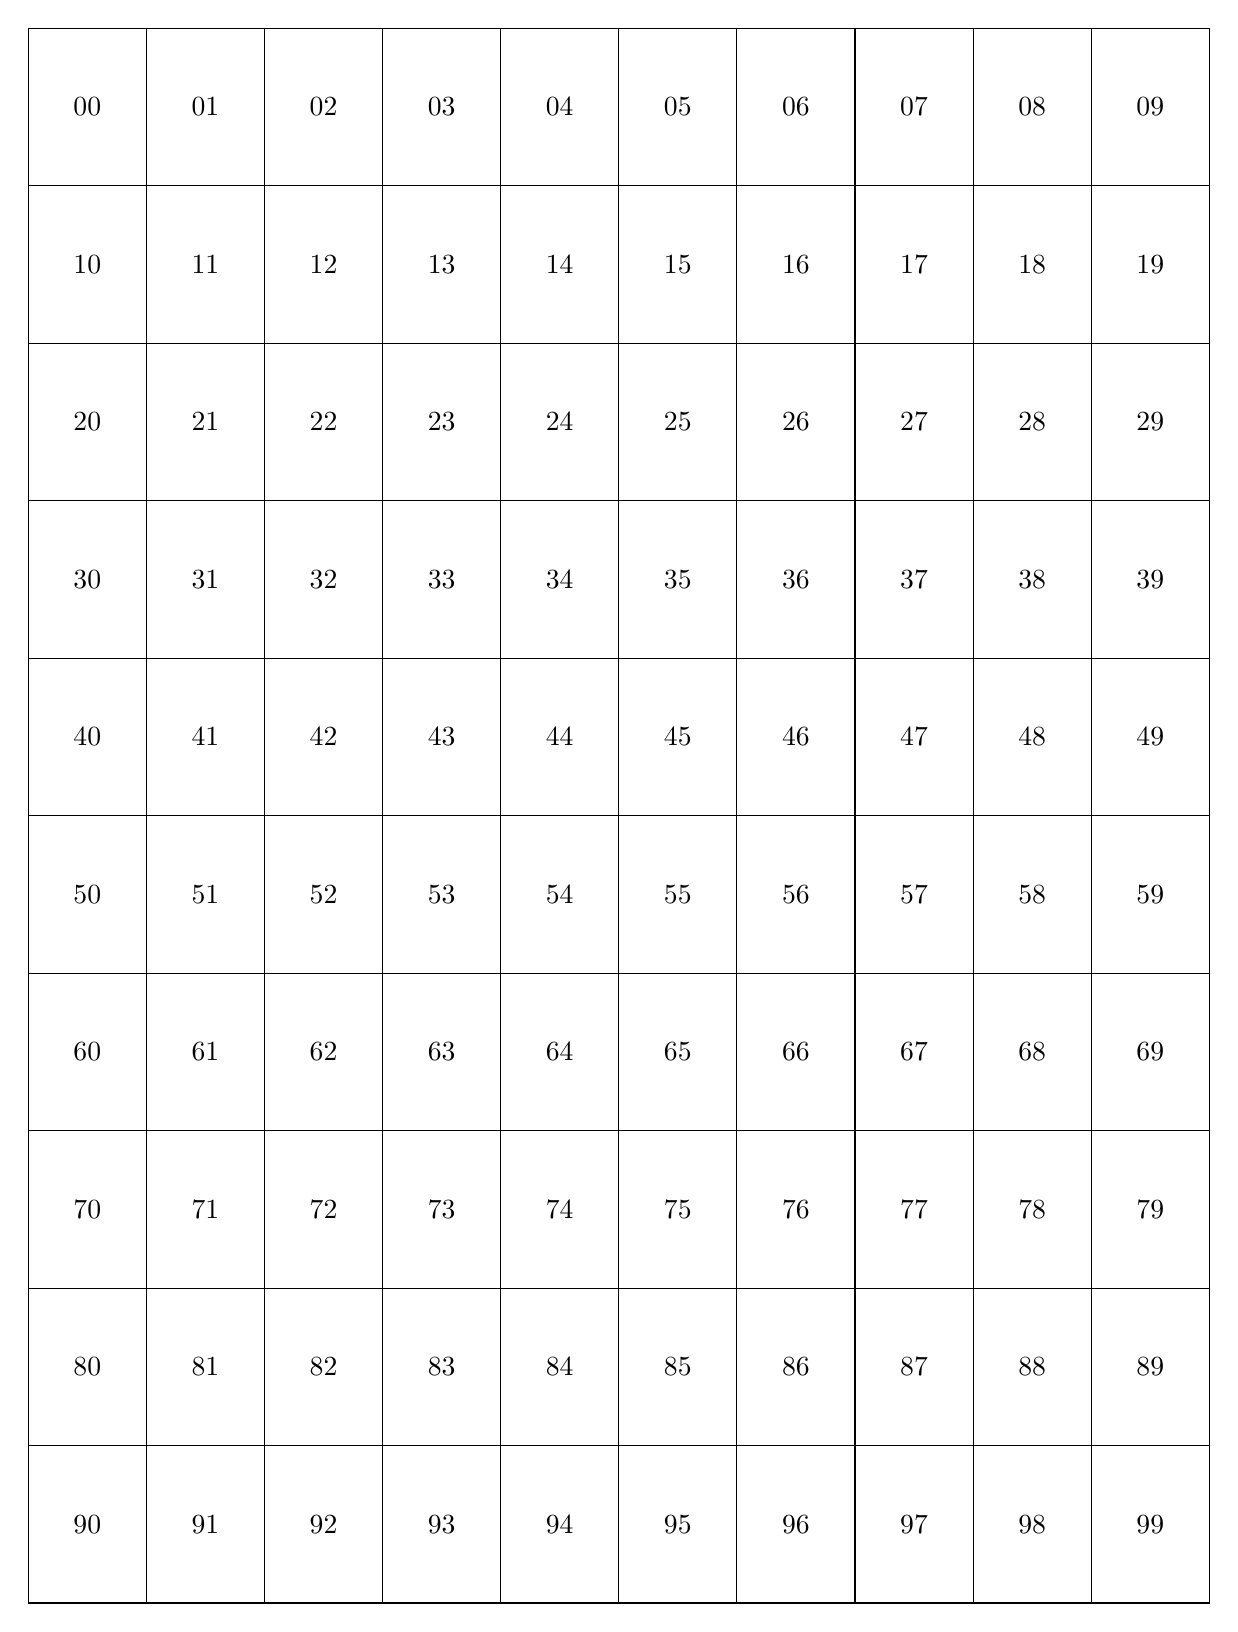
\begin{tikzpicture}
\foreach \y in{0,1,...,9}{
	\foreach \x in {0,1,...,9}{
		\newcommand{\num}{\y \x}
		\draw[black, thin](1.5*\x,-2*\y) rectangle (1.5*\x+1.5,-2*\y-2)node[midway]{\num};
		}
	
	}
\end{tikzpicture}
\end{center}

\newpage
\begin{figure}[!h]
	\centering
	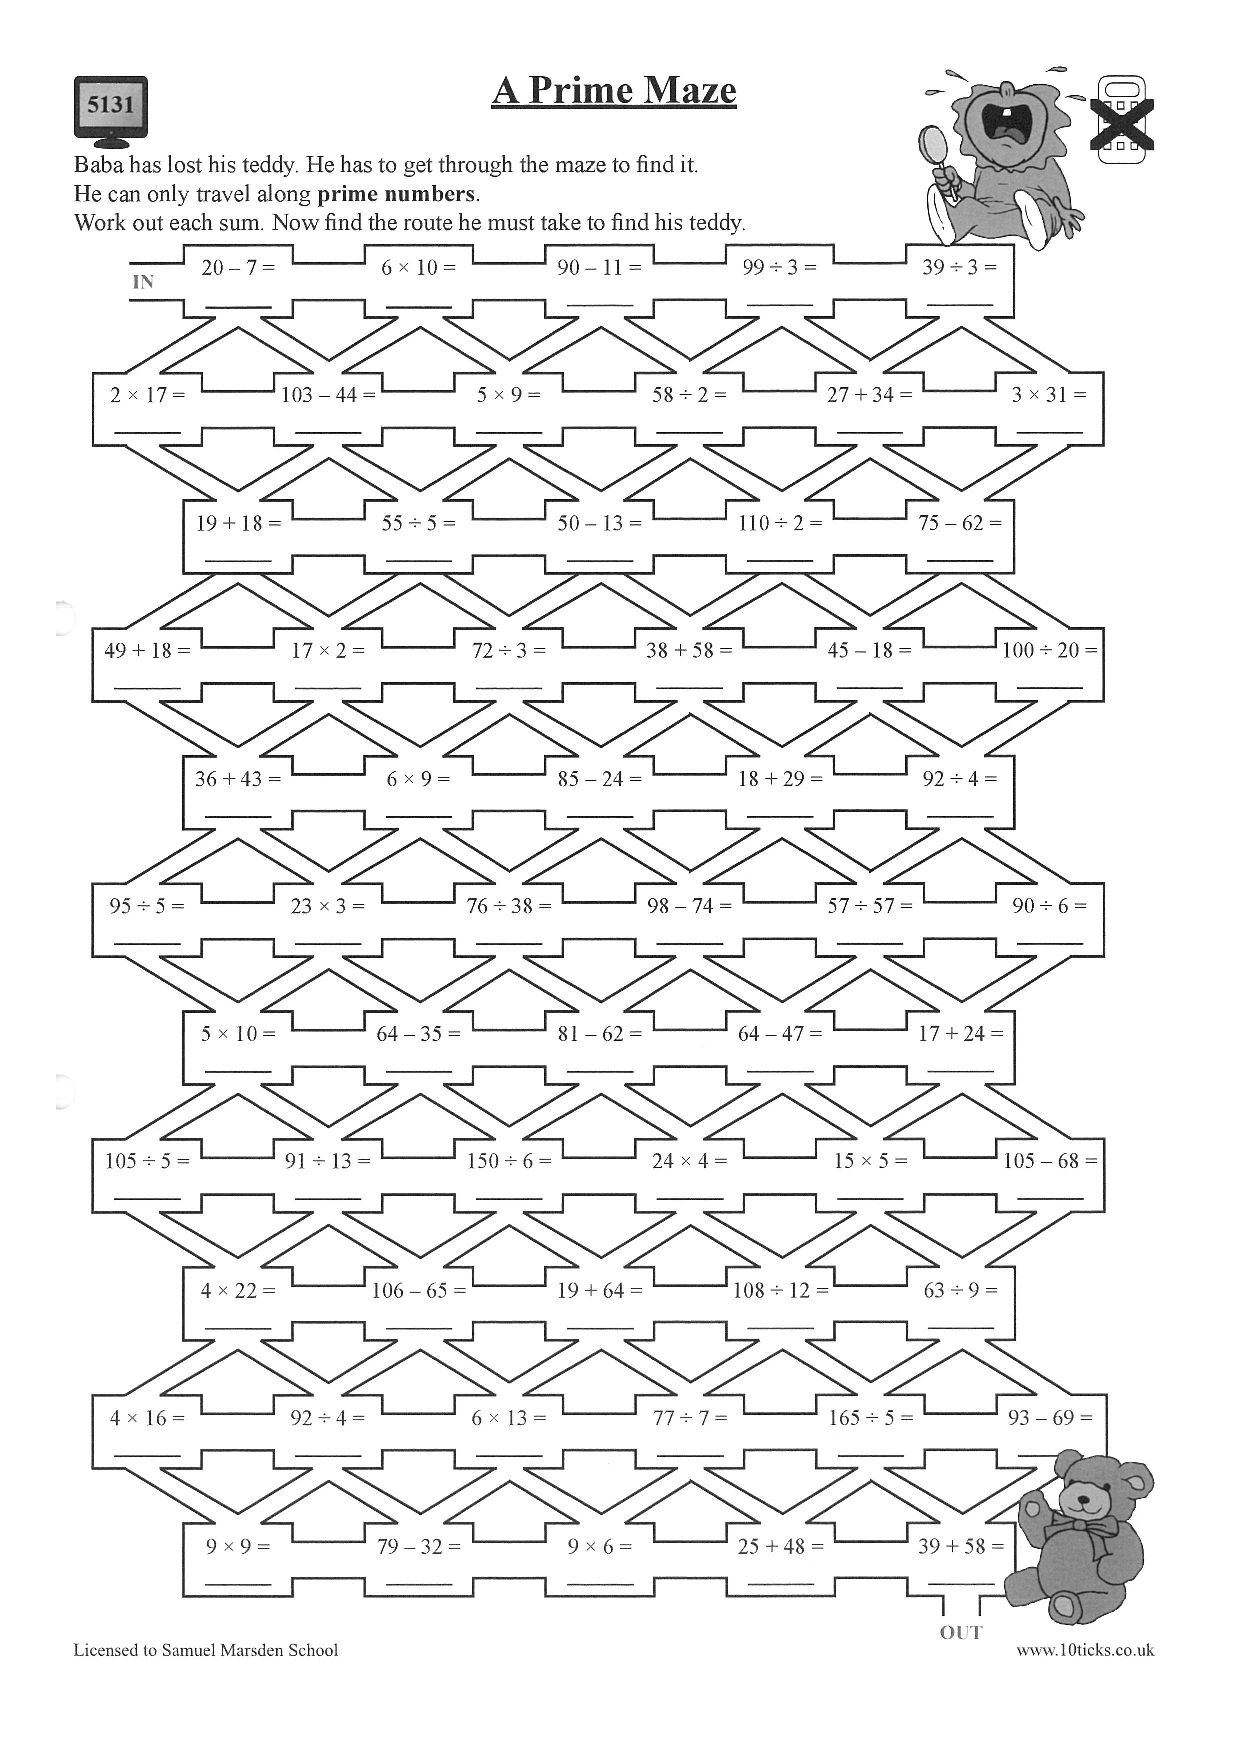
\includegraphics[width=17cm]{Prime_Maze_TT}
\end{figure}
\newpage
\section{Factors:}
To find factors or a number we can write a \textbf{\underline{factor list}} or we can make a \textbf{\underline{factor tree}}.
\subsection{Factor Lists}
To make a factor list for the number 36, we start with:
\begin{align*}
&1,36&&\text{\textit{(because $1\times 36=36$)}}\\
&2,18&& \\
&3,12&&\\
&4,9&&\\
&6,6&&\text{\textit{(we don't need to go further because they will repeat)}}\\               
\end{align*}
\begin{tcolorbox}[colback=red!0!white, colframe=gray ,title=\subsubsection{Write factor lists for:}\label{factorlists}]
\begin{multicols}{4}
	\begin{enumerate}[label= \roman*)]
	 \item 24 
	 \item 30     
	 \item 48       
	 \item 84     
	 \item 96    
	 \item 221   
	 \item 210
	\end{enumerate}
\end{multicols}
\end{tcolorbox}\vspace{0.75cm}

\subsection{Factor Trees and the Product of Prime Factors}
To make a factor tree we start with a number at the top and then find any two factors of the number and put these as branches. We then find factors of each of those numbers.\\ 
If the number is prime we cannot add a branch.\\
This is an example of a factor tree for the number 40:
\begin{center}
	

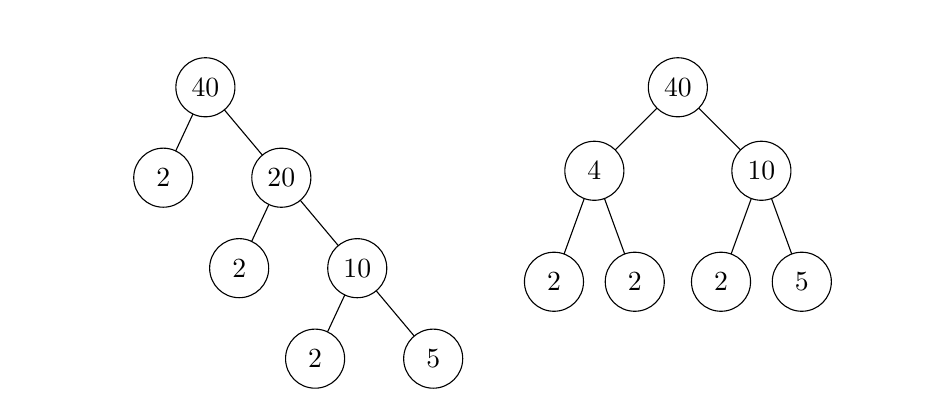
\begin{tikzpicture}[scale=0.75]
\draw[white, thin](0,9) rectangle (15,3);
\coordinate (A) at (3,8);
\coordinate (B) at ([shift=(-50:2)] A);
\coordinate (C) at ([shift=(-50:2)] B);
\coordinate (D) at ([shift=(-50:2)] C);
\coordinate (E) at ([shift=(180:2)] D);
\coordinate (F) at ([shift=(130:2)] E);
\coordinate (G) at ([shift=(130:2)] F);
\draw[black,thin](A)--(B);
\draw[black,thin](A)--(G);
\draw[black,thin](B)--(C);
\draw[black,thin](B)--(F);
\draw[black,thin](C)--(D);
\draw[black,thin](C)--(E);
   \newcommand{\vertB}{A,B,C,D,E,F,G}
  \def\numS{{0,40,20,10,5,2,2,2}}
\foreach \coord [count=\i] in \vertB{
   	\pgfmathsetmacro{\pa}{\numS[\i]}
   	\filldraw[fill=white, draw=black,thin] (\coord) circle[radius=0.5]node[]{\pa};
   }
%------------------
\coordinate (H) at (11,8);
\coordinate (I) at ([shift=(-45:2)] H);
\coordinate (J) at ([shift=(-135:2)] H);
\coordinate (K) at ([shift=(-70:2)] I);
\coordinate (L) at ([shift=(-110:2)] I);
\coordinate (M) at ([shift=(-70:2)] J);
\coordinate (N) at ([shift=(-110:2)] J);
\draw[black,thin](H)--(I);
\draw[black,thin](H)--(J);
\draw[black,thin](I)--(K);
\draw[black,thin](I)--(L);
\draw[black,thin](J)--(M);
\draw[black,thin](J)--(N);
   \newcommand{\vertQ}{H,I,J,K,L,M,N}
   \def\numSet{{0,40,10,4,5,2,2,2}}
   \foreach \coord [count=\i] in \vertQ{
   	\pgfmathsetmacro{\pa}{\numSet[\i]}
   	\filldraw[fill=white, draw=black,thin] (\coord) circle[radius=0.5]node[]{\pa};
   }
\end{tikzpicture}
\end{center}
Both of these trees are correct because we get the same prime numbers at the end.\\\\
From the tree we can find the prime numbers (at the ends of the branches)\\ that multiply to make 40.\\   $2\times 2\times 2\times 5=40$   \\or   $2^{3}\times 5=40$ \\  (this is writing 40 as a product of prime factors).\\
\begin{tcolorbox}[colback=red!0!white, colframe=gray ,title=\subsubsection{Draw Factor Trees for the following numbers and write the numbers as a product of prime factors:}\label{factortrees}]

\begin{multicols}{4}
	\begin{enumerate}[label= \roman*)]
		\item 24 
		\item 30     
		\item 48       
		\item 84     
		\item 96    
		\item 221   
		\item 210
	\end{enumerate}
\end{multicols}
\end{tcolorbox}\vspace{1cm}
 
\section{Highest Common Factor}
\textbf{The Highest Common Factor (HCF) of any 2 (or more) numbers is the largest number that is a factor of those numbers.}\\\\
For example, the HCF of 12 and 18 is 6 (other common factors are 1, 2 and 3 but these are not the highest).
\subsection{Finding HCF using Factor Lists:}
To find HCF of 2 numbers we can write a factor list and find the highest number in both lists.\\\\
For example, what is the HCF of 36 and 96?\\
\footnotesize
\begin{tabular}{|m{2cm}|m{2cm}||m{2cm}|m{2cm}|}\hline
	\multicolumn{2}{|c||}{Factors of 36}&\multicolumn{2}{c|}{Factors of 96}\\\hline
1&	36&	1&	96\\\hline
2&	18&	2&	48\\\hline
3&	\textbf{12}&	3&	32\\\hline
4&	9&	4&	24\\\hline
6&	6&	6&	16\\\hline
&&8&	\textbf{12}       \\\hline
\end{tabular}
\begin{tabular}{|m{5cm}|}\hline
12 is the highest number in both lists.\\
So it is the highest common factor of 36 and 96.\\
HCF(36,96)=12\\\hline
\end{tabular}\vspace{0.5cm}
\normalsize
\begin{tcolorbox}[colback=red!0!white, colframe=gray ,title=\subsubsection{Using Factor Lists, find the Highest Common Factor for:}\label{hcf1}]

\begin{multicols}{4}
	\begin{enumerate}[label= \roman*)]
		\item 48 , 54
		\item 96, 120
		\item 64, 32
		\item 120, 160
	\end{enumerate}
\end{multicols}
\end{tcolorbox}\vspace{0.5cm}

\subsection{Finding HCF using Venn Diagrams:}
We can use Venn Diagrams to find the HCF of 24 and 36.
We write each number as a product of prime factors (using a factor tree if necessary):
\begin{align*}
24=2\times 2\times 2\times 3\\
36=2\times 2\times 3\times 3
\end{align*}
\begin{multicols}{2}
	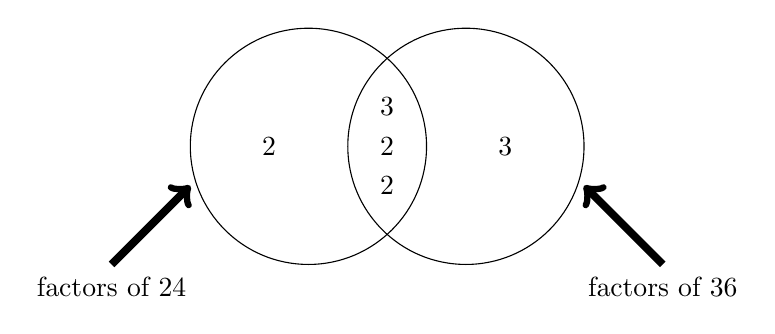
\begin{tikzpicture}

	\draw[black, thin](3,2) circle[radius=1.5];
	\draw[black, thin](5,2) circle[radius=1.5];
	\node at (4,1.5){2};
		\node at (4,2){2};
			\node at (4,2.5){3};
			\node at (2.5,2){2};
			\node at (5.5,2){3};
\draw[black , line width=1mm, ->](0.5,0.5)node[below]{factors of 24}--(1.5,1.5);
\draw[black , line width=1mm, ->](7.5,0.5)node[below]{factors of 36}--(6.5,1.5);	
	\end{tikzpicture}\\\\
By multiplying the prime factors that are \underline{common to both} we find the Highest Common Factor of 24 and 36.\\\\
So $HCF(24,36)=2\times 3\times 2=12$
\end{multicols}
\begin{tcolorbox}[colback=red!0!white, colframe=gray ,title=\subsubsection{For the following pairs of numbers, write them as a product of prime factors and then draw Venn Diagrams to find their Highest Common Factor.}\label{hcfVenn}]
\begin{multicols}{4}
\begin{enumerate}[label= \roman*)]
\item 32, 48
\item 48, 54
\item 64, 84
\item 72, 96
\end{enumerate}
\end{multicols}
\end{tcolorbox}\vspace{1cm}
\section{Multiples}
A multiple of a number is any number we get when the number is multiplied by a whole number.\\
\textbf{For Example:}
the multiples of 4 are: 4, 8, 12, 16, 20, 24, 28, …\\\\
Numbers can “share” multiples  (e.g 24 is a multiple of 2,3,4,6,8,12) and these are called “common multiples”.\\
Some common multiples of 6 and 5 are 30, 60, 90, …\\\\
\textbf{The least or Lowest Common Multiple (LCM) of 2 numbers is the first common multiple we can find.}\\
For example the LCM of 2 and 5 is 10.
\subsection{Finding the LCM by listing multiples:}
To find it we can write out the multiples of both and then find the first common one:\\\\
\textbf{For example find the LCM of 4 and 5:}\\\\
\textbf{Multiples of 4: }  4,  8, 12, 16,  20,  24, 28 , 32 ,36,..\\
\textbf{Multiples of 5: }  5, 10,  15, 20, 25, 30,…\\\\
20 is the first multiple that is shared by both, so 20 is the lowest common multiple of 4 and 5.\\
\textbf{LCM(4,5)=20}\\\\
\begin{tcolorbox}[colback=red!0!white, colframe=gray ,title=\subsubsection{Find the LCM of:}\label{LCM}]
\begin{multicols}{5}
	\begin{enumerate}[label= \roman*)]
		\item 15, 10   
		\item 20, 24   
		\item 16, 28
		\item 14, 21
		\item 19, 6
	\end{enumerate}
\end{multicols}
\end{tcolorbox}\vspace{0.25cm}
\subsection{Finding the LCM using Venn Diagrams:}
Find the LCM of 16 and 24.  (express as product of prime factors).
\begin{align*}
16=2\times 2\times 2\times 2\\
24=2\times 2\times 2\times 3
\end{align*}
\begin{multicols}{2}
	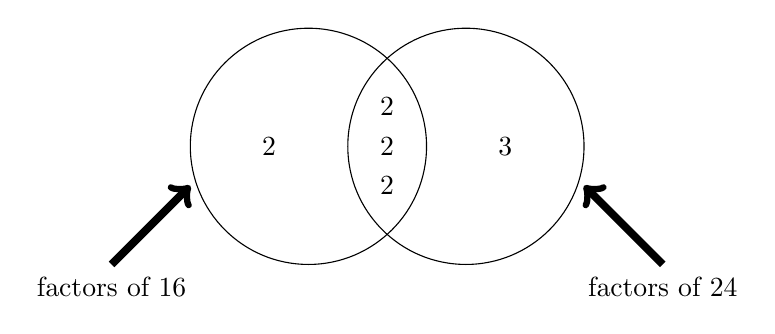
\begin{tikzpicture}
	
	\draw[black, thin](3,2) circle[radius=1.5];
	\draw[black, thin](5,2) circle[radius=1.5];
	\node at (4,1.5){2};
	\node at (4,2){2};
	\node at (4,2.5){2};
	\node at (2.5,2){2};
	\node at (5.5,2){3};
	\draw[black , line width=1mm, ->](0.5,0.5)node[below]{factors of 16}--(1.5,1.5);
	\draw[black , line width=1mm, ->](7.5,0.5)node[below]{factors of 24}--(6.5,1.5);	
	\end{tikzpicture}\\\\
This time we multiply all the numbers in the Venn Diagram together.\\\\
$LCM(16,24)=2\times 2\times 2\times 2\times 3=48$\\
\end{multicols}
\begin{tcolorbox}[colback=red!0!white, colframe=gray ,title=\subsubsection{For the following pairs of numbers, write them as a product of prime factors and then draw Venn Diagrams to find their Lowest Common Multiple.}\label{LCMVenn}]
\begin{multicols}{4}
	\begin{enumerate}[label= \roman*)]
		\item 12, 18   
		\item 32, 52   
		\item 64, 100
		\item 210, 200
	\end{enumerate}
\end{multicols}
\end{tcolorbox}



\newpage
\section{Further Questions}
\begin{tcolorbox}[colback=red!0!white, colframe=gray ,title=\subsection{Set One}\label{SetOne}]
\begin{enumerate}
	\item For each pair of numbers, express them as a product of prime factors and use Venn Diagrams to find their HCF.
	\begin{enumerate}
		\item 24,56
		\item 27,36
		\item 96,120
		\item 60,252
	\end{enumerate}
\item A number``A'' has prime factors : 2,2,3,7,13,13,19 , and ``B'' has prime factors 2,3,7,7,13,19,19.
\begin{enumerate}
	\item Find the two numbers A and B and use Venn Diagrams to find their HCF.
\end{enumerate}
\item	Do the same for:
\begin{enumerate}
	\item A: 2,2,3,5,13,17,5~~~~~~B: 2,3,3,5,17,7
	\item A: 2,3,13,17,17,23,13,5~~~~~~B: 17,3,23,5,2,2,2,5
\end{enumerate}
\item A has prime factors 2,3,3,5,7,7  , B has prime factors 2,2,2,3,7 and C has prime factors 2,2,3,5,7,
\begin{enumerate}
	\item What is HCF(A,B,C)?
	\item What is LCM(A,B,C)?
\end{enumerate}
\end{enumerate}
\end{tcolorbox}
\begin{tcolorbox}[colback=red!0!white, colframe=gray ,title=\subsection{Set Two}\label{SetTwo}]
\begin{enumerate}
	\item Pencils come in packages of 10. Erasers come in packages of 12. Miranda wants to purchase the smallest number of pencils and erasers so that she will have exactly one eraser per pencil. How many packages of pencils and erasers should Miranda buy?\\
	A. 4 packages of pencils and 3 packages of erasers.\\
	B. 5 packages of pencils and 4 packages of erasers.\\
	C. 6 packages of pencils and 5 packages of erasers.\\
	D. 12 packages of pencils and 10 packages of erasers.
	\item Kiara baked 30 oatmeal cookies and 48 chocolate chip cookies to package in plastic containers for her friends at school. She wants to divide the cookies into identical containers so that each container has the same number of each kind of cookie. She wants the largest number of containers possible. How many plastic containers does she need?
	\item Boxes that are 12 inches tall are being stacked next to boxes that are 18 inches tall.
	\begin{enumerate}
		\item What is the shortest height at which the two stacks will be the same height?
	    \item What are some other possible heights at which the two stacks will be the same height?
	\end{enumerate}
\end{enumerate}
\end{tcolorbox}
\begin{tcolorbox}[colback=red!0!white, colframe=gray ,title=\subsection{Set Three}\label{SetThree}]
\begin{enumerate}
	\item Beginning at 8:30AM, tours of the National Capitol and the White House begin. Tours for the National Capitol leave every 15 minutes. Tours for the White House leave every 20 minutes. How often do the tours leave at the same time?\\
	A. Every 15 minutes\\
	B. Every 30 minutes\\
	C. Every 45 minutes\\
	D. Every 60 minutes
	\item Explain the difference between listing the factors of a number and listing the multiples of a number.\\
	\item Two neon lights are turned on at the same time. One blinks every 4 seconds and the other blinks every 6 seconds. In 60 seconds, how many times will they blink at the same time?\\
	\item Bridget has swimming lessons every fifth day and diving lessons every third day. If she had a swimming lesson and a diving lesson on May 5, when will be the next date on which she has both swimming and diving lessons?
	\item The table shows the number of students in the school choir.
	\begin{multicols}{2}
\begin{center}
			\begin{tabular}{|c|c|}\hline
				\multicolumn{2}{|c|}{School Choir}\\\hline
				Student&Number\\\hline
				Girls&48\\\hline
				Boys&64\\\hline
			\end{tabular}\columnbreak
\end{center}
			The choir teacher plans to arrange the students in equal rows.\\ Only girls or boys will be in each row.\\ What is the greatest number of students that could be in each row?\\
			A: 16~~~~~B: 12~~~~~C: 8~~~~~D: 4
	\end{multicols}
	\item At a display booth in an amusement park, every visitor gets a gift bag. Some of the bags have items in them as shown on this table.
\begin{center}
	\begin{tabular}{|l|l|}\hline
		\multicolumn{2}{|c|}{Items in the Gift Bags}\\\hline
		\textbf{Items}&\textbf{Bags}\\\hline
		Hat&Every $2^{nd}$ Visitor\\\hline
		T-shirt&Every $7^{th}$ Visitor\\\hline
		Backpack&Every $10^{th}$ Visitor\\\hline
	\end{tabular}
\end{center}
How often will the bag contain all 3 items?

\item Hot dogs come in packages of 8. Hot dog buns come in packages of 12. If Grace wants to have enough to serve 24 people and have none left over, how many packages of hot dogs and hot dog buns should she purchase? 
\end{enumerate}
\end{tcolorbox}\vspace{0.75cm}
\begin{tcolorbox}[colback=red!0!white, colframe=gray ,title=\subsection{Set Four - more difficult questions}\label{SetFour}]
\begin{enumerate}
	\item Jack can paint a house in 5 days, while Jill can paint the same house in 7 days. How long will it take them to paint one house working together?
\item It takes Bill 3 hours to load a truck with firewood, Jane 5 hours to do the same job and Jonny can load the truck in 6 hours. How long on hours and minutes would it take the three of them working together?
\item Two ferry boats travel between Auckland and Devonport. They leave from the two terminals at the same time, with one leaving Auckland taking 12 minutes to Devonport, while the one leaving Devonport takes 10 minutes to get to Auckland. How long will it be before they meet?
\item Two athletes decide to run the 400m track in different directions. If athlete A runs 400m in 52 seconds and athlete B runs 400m in 48 seconds, how long will be before they meet each other? How far has each runner covered?
\item If the hot tap can fill a bath in 8 minutes, while the cold tap can fill the bath in 10 minutes, how long will it take both taps to fill the bath if they are turned on together (and the plug is in)?
\item Pat and Andy working together can complete a job in 9 hours. Pat knows he can do the job by himself in 15 hours. how long would it take Andy, working by himself?
\item Two trains leave Auckland and Wellington simultaneously. The train going to Auckland can complete the journey in 12 hours while the one leaving Wellington can complete the journey in 16 hours. After how long will they meet?
\item Two trains travelling simultaneously between the same two stations in opposite directions meet after they have been travelling 3 hours. If they began their journey's together and one train can complete the whole journey in 5 hours, how long does it take the other train to complete the full journey?
\end{enumerate}
\end{tcolorbox}
\newpage
\section{Integers}
\subsection{Introduction}\label{submalloon}

\begin{figure}[!h]
	\centering
	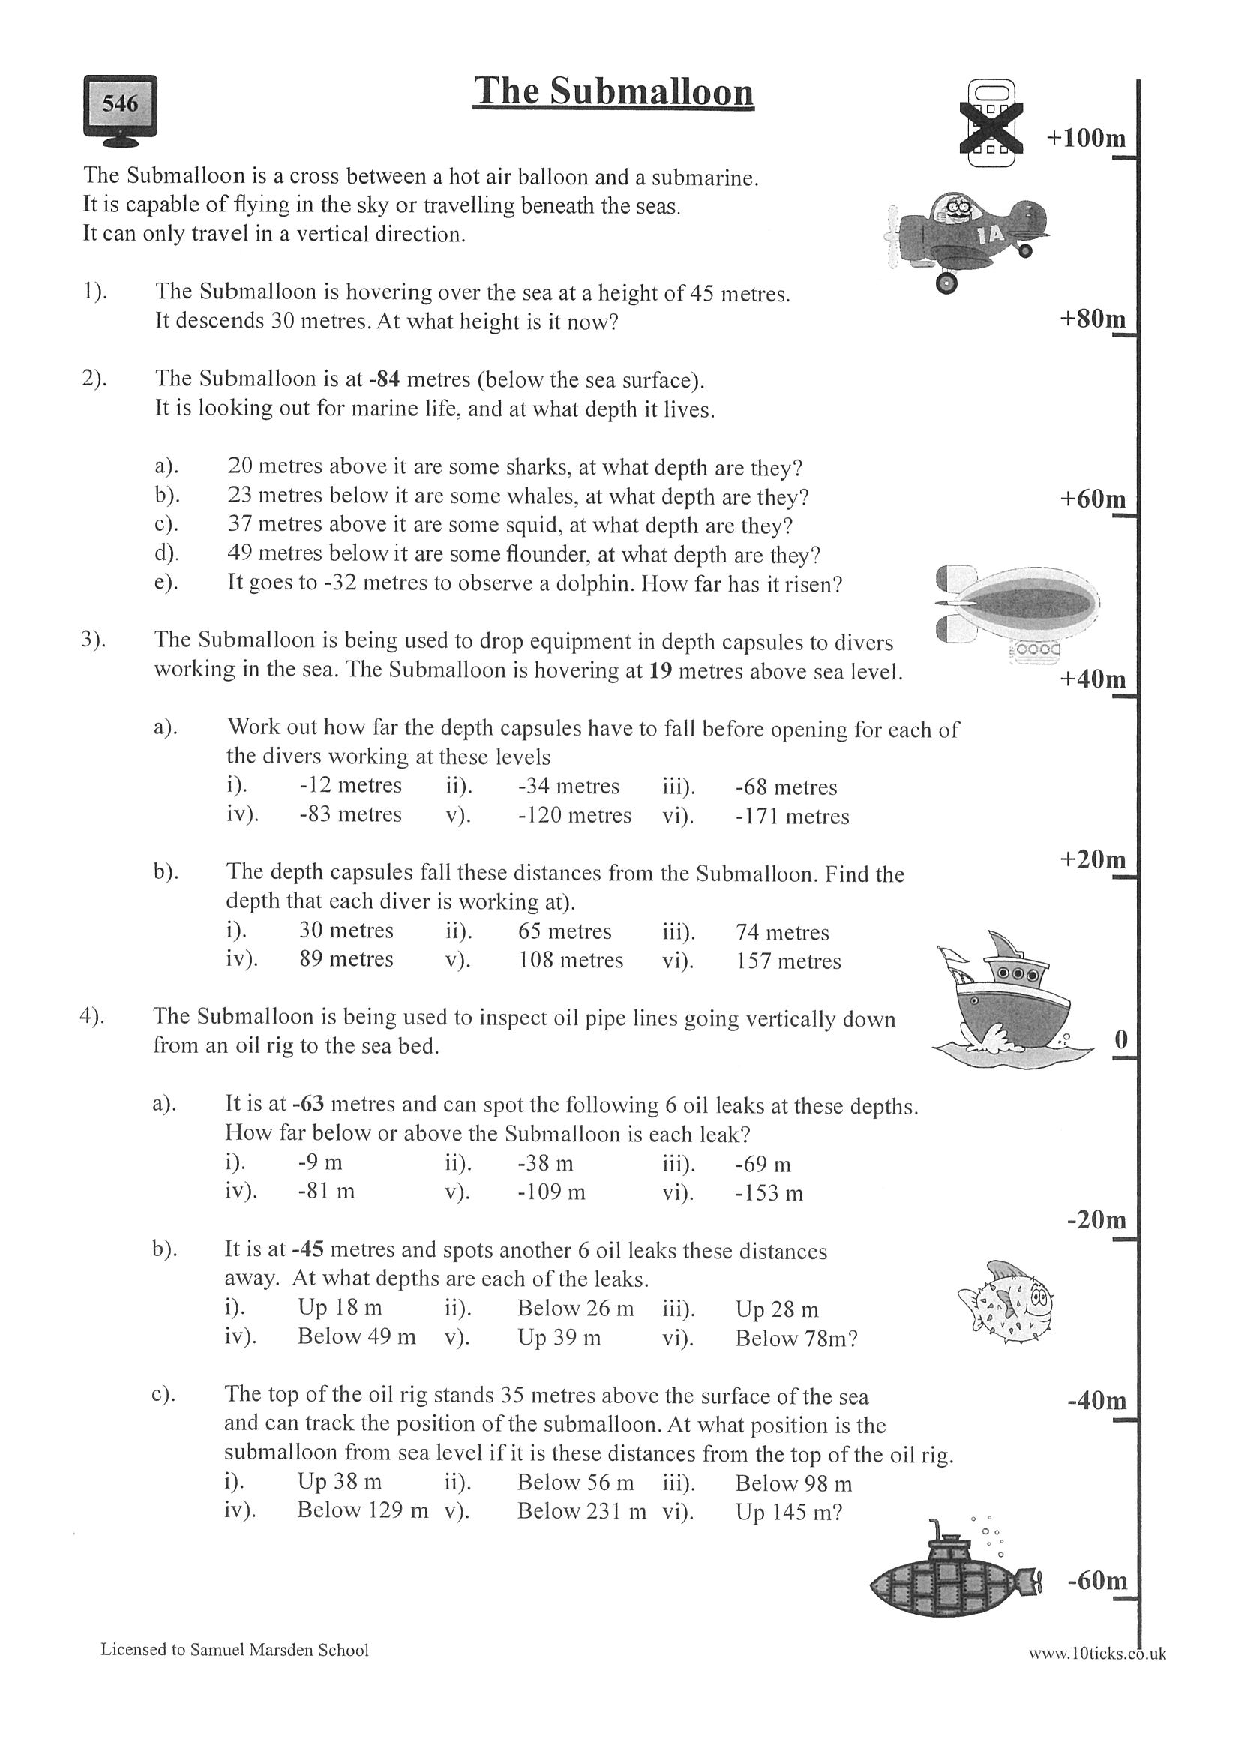
\includegraphics[width=17cm]{Submalloon}
	% \caption{a nice plot}
	 %\label{fig:mesh1}
\end{figure}


\newpage
\subsection{Definition of integers}
\begin{onehalfspace}
When a number line starts at 0 and moves to the right. The numbers are \textbf{positive} numbers.\\
If we are only using the numbers 0,1,2,3,4,5,... then we have \textbf{Whole Numbers}.\\
The proper term for Whole Numbers is \textbf{Natural Numbers}. \\
The symbol is $\mathbb{N}$. 
\begin{center}
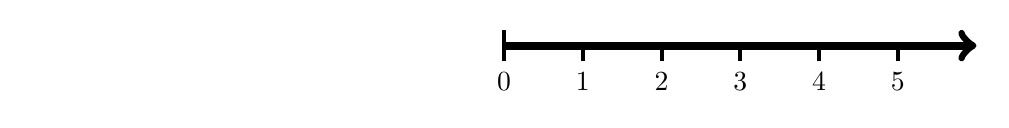
\begin{tikzpicture}
\draw[black, line width=1mm, ->](0,0)--(6,0);
\draw[white, line width=1mm, ->](0,0)--(-6,0);
\draw[black, ultra thick](0,-0.2)--(0,0.2);
\foreach \x in {0,1,...,5}{
	\draw[black, line width=0.5mm](\x,0)--(\x,-0.2)node[below]{\x };
	}
\end{tikzpicture}
\end{center}
If we extend the number line to the left, we now have negative numbers.\\
All whole positive and negative numbers are called \textbf{Integers}. \\
The symbol is $\mathbb{Z}$.
\begin{center}
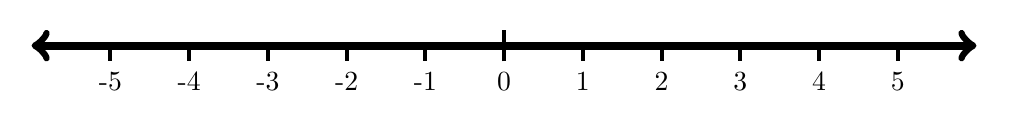
\begin{tikzpicture}
\draw[black, line width=1mm, ->](0,0)--(6,0);
\draw[black, line width=1mm, ->](0,0)--(-6,0);
\draw[black, ultra thick](0,-0.2)--(0,0.2);
\foreach \x in {-5,-4,...,5}{
	\draw[black, line width=0.5mm](\x,0)--(\x,-0.2)node[below]{\x };
}
\end{tikzpicture}
\end{center}\vspace{0.5cm}
\begin{tcolorbox}[colback=red!0!white, colframe=gray ,title=\subsubsection{Use a number line (when you need to), to help you work out the following sums.}\label{IntOne}]
\begin{multicols}{3}
	\begin{enumerate}[label=\footnotesize \roman*)]
		\item~~~$3+5=$
		\item~~~$3-5=$
		\item~~~$2+8=$
		\item~~~$2-8=$
		\item~~~$1+12=$
		\item~~~$1-12=$
		\item~~~$4+9=$
		\item~~~$4-9=$
		\item~~~$7+14=$
		\item~~~$7-14=$
		\item~~~$18+\square=45$
		\item~~~$18-\square=-9$
	\end{enumerate}
\end{multicols}
\end{tcolorbox}\vspace{0.5cm}
\begin{tcolorbox}[colback=red!0!white, colframe=gray ,title=\subsubsection{Use a number line (when you need to), to help you work out the following sums.}\label{IntTwo}]
\begin{multicols}{3}
	\begin{enumerate}[label=\footnotesize \roman*)]
		\item~~~$-3+5=$
		\item~~~$-3-5=$
		\item~~~$-2+8=$
		\item~~~$-2-8=$
		\item~~~$-1+12=$
		\item~~~$-1-12=$
		\item~~~$-4+9=$
		\item~~~$-4-9=$
		\item~~~$-7+14=$
		\item~~~$-7-14=$
		\item~~~$-18+\square=-5$
		\item~~~$-18-\square=-50$
	\end{enumerate}
\end{multicols}
\end{tcolorbox}\vspace{0.5cm}
\begin{tcolorbox}[colback=red!0!white, colframe=gray ,title=\subsubsection{Use a number line (when you need to), to help you work out the following sums.}\label{IntThree}]
\begin{multicols}{3}
	\begin{enumerate}[label=\footnotesize \roman*)]
		\item~~~$-13+5=$
		\item~~~$9-12=$
		\item~~~$-2+1=$
		\item~~~$-2+0=$
		\item~~~$-15+6=$
		\item~~~$-18-30=$
		\item~~~$-21+24=$
		\item~~~$-70-9=$
		\item~~~$-70+9=$
		\item~~~$-70-24=$
		\item~~~$-70+\square=-46$
		\item~~~$-70+\square=34$
	\end{enumerate}
\end{multicols}
\end{tcolorbox}





\newpage		
\subsection{Adding and Subtracting Integers}
If we write the number ``5'' it is implied that it is positive so we could write it as $^{+}5$\\\\
So: \Large $^{+}5+^{+}7=5+7=12$\\
\normalsize This means we start at 5 and move 7 spaces up the number line.\\
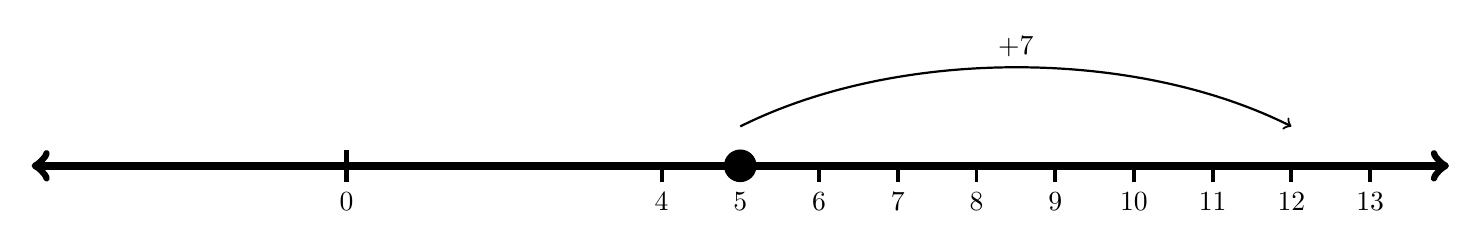
\begin{tikzpicture}
\draw[black, line width=1mm, ->](0,0)--(14,0);
\draw[black, line width=1mm, ->](0,0)--(-4,0);
\draw[black, ultra thick](0,0.2)--(0,-0.2)node[below]{0};
\filldraw [black](5,0) circle[radius=2mm];
\foreach \x in {4,5,...,13}{
	\draw[black, line width=0.5mm](\x,0)--(\x,-0.2)node[below]{\x };
}
\draw[black, thick, ->](5,0.5).. controls (7,1.5) and (10,1.5)..(12,0.5)node[midway, above]{+7};
\end{tikzpicture}\\\\
If we ``add'' $^{-}7$ we are going in the opposite direction to the $^{-}7$\\\\ 
So: \Large $^{+}5+^{-}7=5-7=-2$\\
\normalsize This means we start at 5 and move 7 spaces up the number line.\\
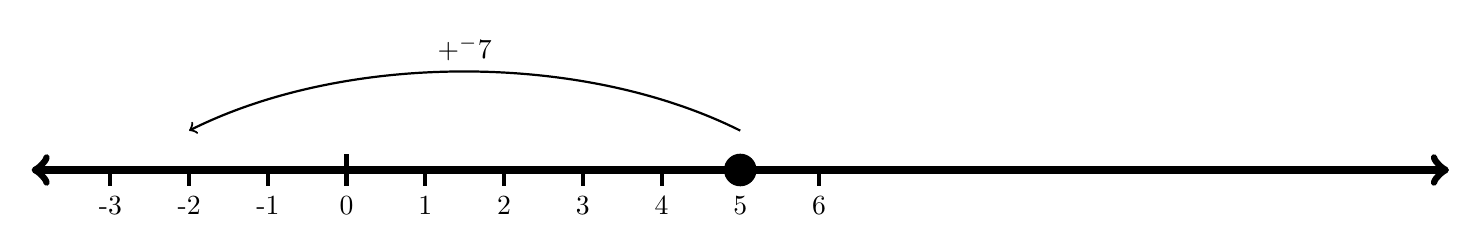
\begin{tikzpicture}
\draw[black, line width=1mm, ->](0,0)--(14,0);
\draw[black, line width=1mm, ->](0,0)--(-4,0);
\draw[black, ultra thick](0,0.2)--(0,-0.2);
\filldraw [black](5,0) circle[radius=2mm];
\foreach \x in {-3,-2,...,6}{
	\draw[black, line width=0.5mm](\x,0)--(\x,-0.2)node[below]{\x };
}
\draw[black, thick, ->](5,0.5).. controls (3,1.5) and (0,1.5)..(-2,0.5)node[midway, above]{$+^{-}7$};
\end{tikzpicture}\\\\
If we subtract $^{+}7$ we are just doing ordinary subtraction.\\\\
So: \Large $^{+}5-^{+}7=5-7=-2$\\
\normalsize This means we start at 5 and move 7 spaces up the number line.\\
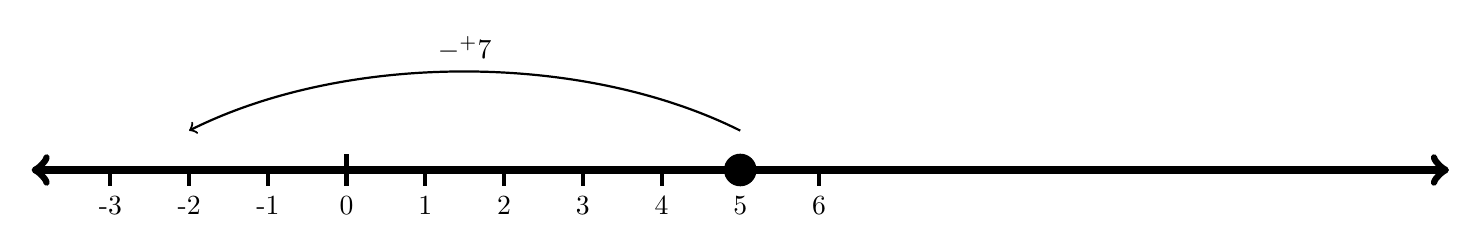
\begin{tikzpicture}
\draw[black, line width=1mm, ->](0,0)--(14,0);
\draw[black, line width=1mm, ->](0,0)--(-4,0);
\draw[black, ultra thick](0,0.2)--(0,-0.2);
\filldraw [black](5,0) circle[radius=2mm];
\foreach \x in {-3,-2,...,6}{
	\draw[black, line width=0.5mm](\x,0)--(\x,-0.2)node[below]{\x };
}
\draw[black, thick, ->](5,0.5).. controls (3,1.5) and (0,1.5)..(-2,0.5)node[midway, above]{$-^{+}7$};
\end{tikzpicture}\\\\
If we subtract $^{-}7$ we are just doing the opposite of the one above.\\\\
So: \Large $^{+}5-^{-}7=5+7=12$\\
\normalsize This means we start at 5 and move 7 spaces up the number line.\\
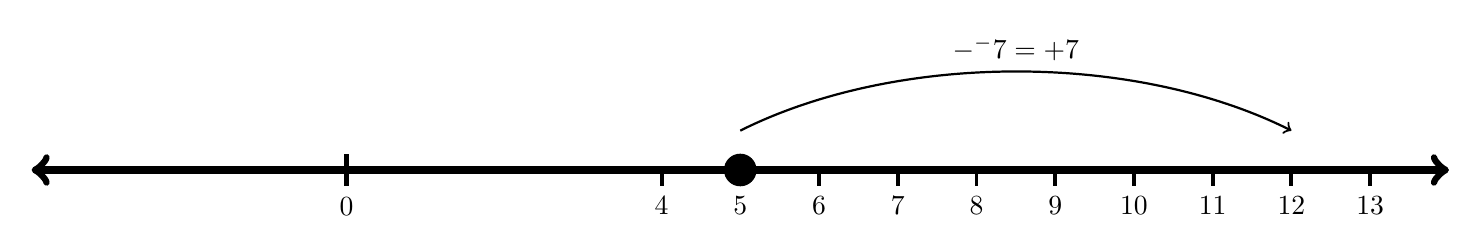
\begin{tikzpicture}
\draw[black, line width=1mm, ->](0,0)--(14,0);
\draw[black, line width=1mm, ->](0,0)--(-4,0);
\draw[black, ultra thick](0,0.2)--(0,-0.2)node[below]{0};
\filldraw [black](5,0) circle[radius=2mm];
\foreach \x in {4,5,...,13}{
	\draw[black, line width=0.5mm](\x,0)--(\x,-0.2)node[below]{\x };
}
\draw[black, thick, ->](5,0.5).. controls (7,1.5) and (10,1.5)..(12,0.5)node[midway, above]{$-^{-}7=+7$};
\end{tikzpicture}\\\\
\end{onehalfspace}
\newpage
We can establish our basic integer addition and subtraction rules:
\begin{align*}
+~+&=+~~~~~~~~~~~\text{\tiny Example:}-7+^{+}9 =-7+9 =2\\\\
+~-&=-~~~~~~~~~~~\text{\tiny Example:} -8+-6=-8-6=-14\\\\
-~+&=-~~~~~~~~~~~\text{\tiny Example:} -3-^{+}14=-3-14=-17\\\\
-~-&=+~~~~~~~~~~~\text{\tiny Example:} -7- -15=-7+15=6\\\\
\end{align*}\vspace{-0.5cm} 
\begin{tcolorbox}[colback=red!0!white, colframe=gray ,title=\subsubsection{Work out the following sums (where necessary, change the two signs in the middle into one sign).}\label{IntFour}]
	\begin{multicols}{3}
		\begin{enumerate}[label=\footnotesize \roman*)]
			\item~~~$3+5=$
			\item~~~$3-5=$
			\item~~~$3+-5=$
			\item~~~$3--5=$
			\item~~~$1+12=$
			\item~~~$1-12=$
			\item~~~$1+-12=$
			\item~~~$1--12=$
			\item~~~$7+14=$
			\item~~~$7-14=$
			\item~~~$7+-14=$
			\item~~~$7--14=$
		\end{enumerate}
	\end{multicols}
\end{tcolorbox}\vspace{0.75cm}
\begin{tcolorbox}[colback=red!0!white, colframe=gray ,title=\subsubsection{Work out the following sums (where necessary, change the two signs in the middle into one sign).}\label{IntFive}]
	\begin{multicols}{3}
		\begin{enumerate}[label=\footnotesize \roman*)]
			\item~~~$-3+5=$
			\item~~~$-3-5=$
			\item~~~$-3+-5=$
			\item~~~$-3--5=$
			\item~~~$-10-6=$
			\item~~~$-10+6=$
			\item~~~$-10--6=$
			\item~~~$-10+-6=$
			\item~~~$-7--14=$
			\item~~~$-7+14=$
			\item~~~$-7-14=$
			\item~~~$-7+-14=$
		\end{enumerate}
	\end{multicols}
\end{tcolorbox}\vspace{0.75cm}
\begin{tcolorbox}[colback=red!0!white, colframe=gray ,title=\subsubsection{General Questions.}\label{IntSix}]
	\begin{multicols}{3}
		\begin{enumerate}[label=\footnotesize \roman*)]
			\item~~~$-12+5=$
			\item~~~$ 16-5=$
			\item~~~$23+-15=$
			\item~~~$30--25=$
			\item~~~$-10--6=$
			\item~~~$22+-30=$
			\item~~~$-45--10=$
			\item~~~$-21-6=$
			\item~~~$-19+-14=$
			\item~~~$-70+14=$
			\item~~~$-9-14=$
			\item~~~$-1--14=$
		\end{enumerate}
	\end{multicols}
\end{tcolorbox}\vspace{0.75cm}
\begin{tcolorbox}[colback=red!0!white, colframe=gray ,title=\subsubsection{In these sums the letter ``A'' stands for a number. Find the correct value of A in each of the sums.}\label{IntSeven}]
	\begin{multicols}{3}
		\begin{enumerate}[label=\footnotesize \roman*)]
			\item~~~$5+A=15$
			\item~~~$ A-5=-2$
			\item~~~$15+A=-6$
			\item~~~$A--6=13$
			\item~~~$0-A=-8$
			\item~~~$0+A=-8$
			\item~~~$-15--A=1$
			\item~~~$-8-A=90$
			\item~~~$-19+2\times A=-3$
			\item~~~$-A+14=-15$
			\item~~~$A-14=-120$
			\item~~~$A--14=-25$
		\end{enumerate}
	\end{multicols}
\end{tcolorbox}\vspace{0.75cm}
\subsubsection{Complete these Addition and Subtraction Grids}
\vspace{0.5cm}
\begin{center}
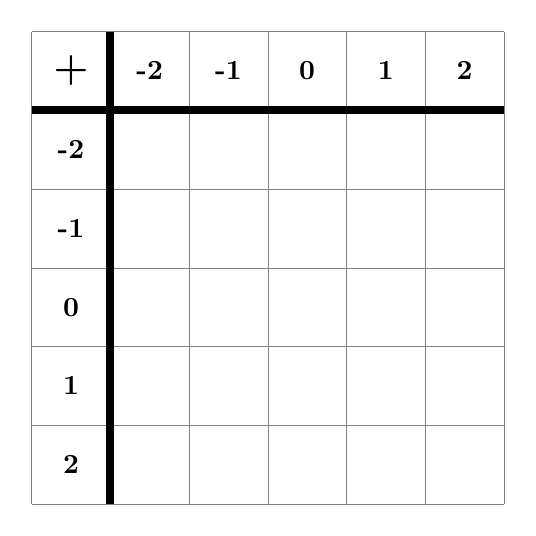
\begin{tikzpicture}
\draw[step=1cm,gray,very thin] (-2,-2) grid (4,4);
\foreach \x in {-2,-1,...,2}{
	\node at (-1.5,-\x+0.5){\textbf{\x}};
	\node at (\x+1.5,3.5){\textbf{\x}};
	}
\node at (-1.5,3.5){\Large \textbf{+}};
\draw[black, line width=1mm](-2,3)--(4,3);
\draw[black, line width=1mm](-1,4)--(-1,-2);
\end{tikzpicture}
\hspace{3cm}
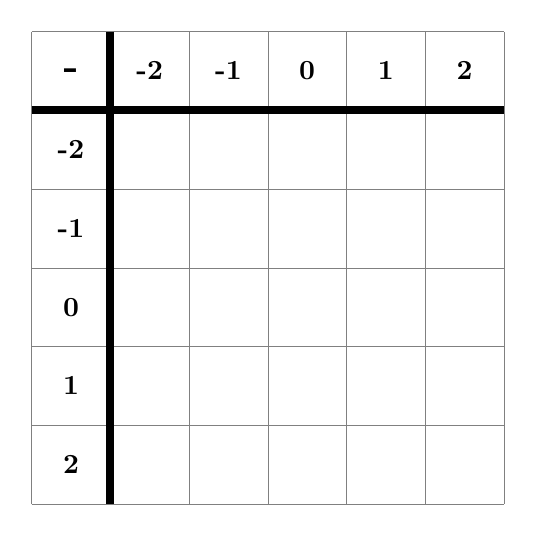
\begin{tikzpicture}
\draw[step=1cm,gray,very thin] (-2,-2) grid (4,4);
\foreach \x in {-2,-1,...,2}{
	\node at (-1.5,-\x+0.5){\textbf{\x}};
	\node at (\x+1.5,3.5){\textbf{\x}};
}
\node at (-1.5,3.5){\Large \textbf{-}};
\draw[black, line width=1mm](-2,3)--(4,3);
\draw[black, line width=1mm](-1,4)--(-1,-2);
\end{tikzpicture}
\end{center}
\vspace{2cm}
\begin{center}
	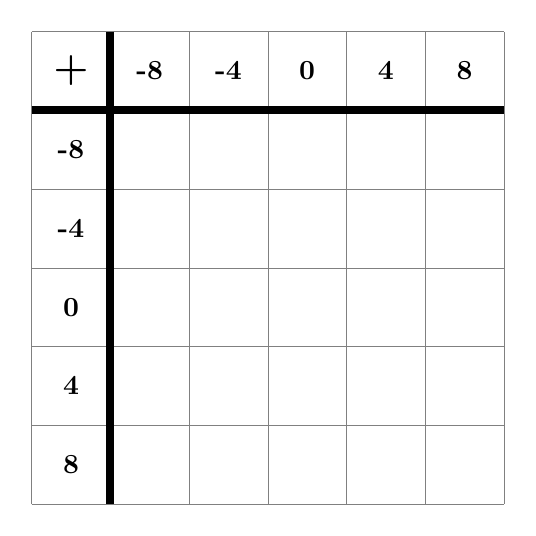
\begin{tikzpicture}
	\draw[step=1cm,gray,very thin] (-2,-2) grid (4,4);
	\foreach \x in {-8,-4,...,8}{
		\node at (-1.5,-\x*0.25+0.5){\textbf{\x}};
		\node at (\x*0.25+1.5,3.5){\textbf{\x}};
	}
	\node at (-1.5,3.5){\Large \textbf{+}};
	\draw[black, line width=1mm](-2,3)--(4,3);
	\draw[black, line width=1mm](-1,4)--(-1,-2);
	\end{tikzpicture}
	\hspace{3cm}
	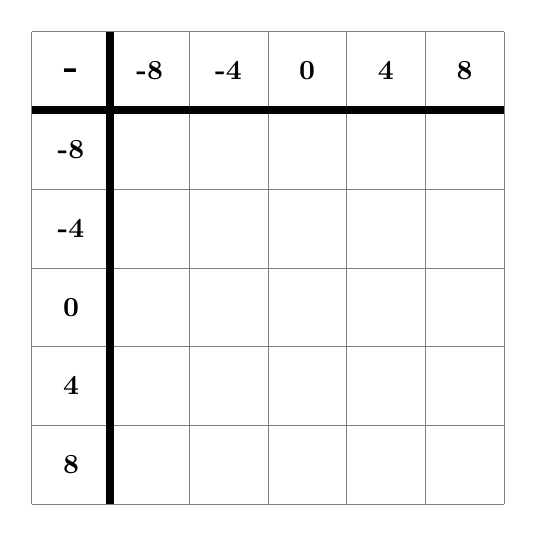
\begin{tikzpicture}
	\draw[step=1cm,gray,very thin] (-2,-2) grid (4,4);
	\foreach \x in {-8,-4,...,8}{
		\node at (-1.5,-\x*0.25+0.5){\textbf{\x}};
		\node at (\x*0.25+1.5,3.5){\textbf{\x}};
	}
	\node at (-1.5,3.5){\Large \textbf{-}};
	\draw[black, line width=1mm](-2,3)--(4,3);
	\draw[black, line width=1mm](-1,4)--(-1,-2);
	\end{tikzpicture}
\end{center}

\newpage

\subsubsection{Addition Pyramids with Negative Numbers}\label{pyramids}
To find the next number, add the two bricks below.
Copy each pyramid and fill in the missing numbers.
\begin{multicols}{3}
\boxes{}{}{}{-7}{9}{6}{1}
\boxes{}{}{}{4}{8}{-10}{4}
\boxes{}{}{}{1}{-5}{7}{2}
\boxes{}{}{}{-9}{-11}{13}{5}
\boxes{}{}{}{-15}{7}{-11}{3}
\boxes{}{}{}{7}{-15}{-6}{6}
\end{multicols}
\begin{multicols}{3}
	\boxes{}{9}{}{5}{}{-7}{7}
	\boxes{-9}{}{1}{}{-3}{}{10}
	\boxes{}{}{-6}{6}{}{-9}{8}
	\boxes{-6}{-1}{}{}{4}{}{11}
	\boxes{}{-7}{}{-9}{}{4}{9}
	\boxes{-24}{}{-21}{}{-15}{}{12}
\end{multicols}
\begin{multicols}{3}
	\boxes{3}{}{}{-7}{}{2}{13}
	\vfill\null
	\columnbreak
	\boxes{-9}{}{}{-11}{}{14}{14}
	\vfill\null
	\columnbreak
	\boxes{-2}{}{}{-8}{}{-10}{15}
\end{multicols}
\newpage
\subsubsection{Magic Squares}\label{magicsquares}
In a magic square, the rows, columns and diagonals all add to the same number (this is the magic number)\\
Complete the following magic squares and find their magic numbers.
\begin{multicols}{3}
\magicsquareA{0,7,2,,3,,,,,1,}
\magicsquareA{1, ,,,3,-2,,,5,4,}
\magicsquareA{0, ,,,1,-3,,,2,2,}
\magicsquareA{ , , , , ,-1,-2,7,1,5,}
\magicsquareA{, ,-2,,-1,,0,,2,3,}
\magicsquareA{ , ,3, ,1,2,-1, , ,6,}
\end{multicols}\vspace{-0.5cm}
\begin{multicols}{3}
	\magicsquareA{ , , ,-7, , , ,-9, -4,7, -15}
	\magicsquareA{-2, ,1, , , ,-7, ,-4,10,}
	\magicsquareA{-8, , , ,-7, ,-3, , ,8, -21}
	\magicsquareA{-5, ,-1, , , ,-7, ,-3,11,}
	\magicsquareA{-5 , ,-7, , , , ,-4, ,9,-24}
	\magicsquareA{3, ,5, , , ,-1, ,1,12,}
\end{multicols}

\newpage
\subsection{Multiplying and Dividing Integers}
\begin{onehalfspace}
We know that $^{+}3$ is the same as 3.\\
So $5\times^{+}3=5\times 3=15$\\
\end{onehalfspace}
Complete the following starting at the top and following the pattern logically into the multiplications of negative numbers.
\begin{align*}
2\times ^{+}4=\\
2\times ^{+}3=\\
2\times ^{+}2=\\
2\times ^{+}1=\\
2\times 0=\\
2\times ^{-}1=\\
2\times ^{-}2=\\
2\times ^{-}3=\\
2\times ^{-}4=
\end{align*}
We can see that if we multiply a positive number by a negative number we will get a negative number as a result.
\begin{align*}
6\times-5=-30
\end{align*}
We also know mulitplication is commutative so: 
\begin{align*}
6\times -5=-5\times 6=-30
\end{align*}
Complete this set starting at the top and following the pattern logically into the multiplications of two negative numbers.
\begin{align*}
-2\times ^{+}4=\\
-2\times ^{+}3=\\
-2\times ^{+}2=\\
-2\times ^{+}1=\\
-2\times 0=\\
-2\times ^{-}1=\\
-2\times ^{-}2=\\
-2\times ^{-}3=\\
-2\times ^{-}4=\\
\end{align*}
\textbf{We can establish our basic integer multiplication rules:}
\begin{align*}
+\times +&= + number~~~~~~~~~~~\text{\tiny Example: }7\times 8 =56\\\\
+\times -&= - number~~~~~~~~~~~\text{\tiny Example: } 9\times ^{-}3=-27\\\\
-\times +&= - number~~~~~~~~~~~\text{\tiny Example: } -8\times ^{+}12=-96\\\\
-\times -&= + number~~~~~~~~~~~\text{\tiny Example: } -7-^{-}9=^{+}63\\\\
\end{align*} 
\newpage
\textbf{Because division is a form of multiplication (it is multiplying by a fraction), the rules for division will be the same.}\\
\begin{align*}
+\div +&= + number~~~~~~~~~~~\text{\tiny Example: }72\div 8 =9\\\\
+\div -&= - number~~~~~~~~~~~\text{\tiny Example: } 36\div^{-}9=-4\\\\
-\div +&= - number~~~~~~~~~~~\text{\tiny Example: } -24\div ^{+}6=-4\\\\
-\div -&= + number~~~~~~~~~~~\text{\tiny Example: } -48-^{-}3=^{+}16\\\\
\end{align*}
\begin{tcolorbox}[colback=red!0!white, colframe=gray ,title=\subsubsection{Work out the following sums.}\label{multInt0}]
	\begin{multicols}{3}
		\begin{enumerate}[label=\footnotesize \roman*)]
			\item~~~$3\times2=$
			\item~~~$3\times-2=$
			\item~~~$-3\times2=$
			\item~~~$-3\times-2=$
			\item~~~$-7\times-8=$
			\item~~~$-7\times8=$
			\item~~~$7\times-8=$
			\item~~~$7\times8=$
			\item~~~$-9\times12=$
			\item~~~$-3\times9=$
			\item~~~$4\times-8=$
			\item~~~$-7\times-9=$
		\end{enumerate}
	\end{multicols}
\end{tcolorbox}\vspace{0.75cm}
\begin{tcolorbox}[colback=red!0!white, colframe=gray ,title=\subsubsection{Work out the following sums.}\label{multInt1}]
	\begin{multicols}{3}
		\begin{enumerate}[label=\footnotesize \roman*)]
			\item~~~$-15\times3=$
			\item~~~$5\times15=$
			\item~~~$4\times-15=$
			\item~~~$-2\times-16=$
			\item~~~$-16\times -3=$
			\item~~~$4\times16=$
			\item~~~$2\times-24=$
			\item~~~$8\times-20=$
			\item~~~$-25\times6=$
			\item~~~$-35\times3=$
			\item~~~$-13\times-3=$
			\item~~~$-14\times3=$
		\end{enumerate}
	\end{multicols}
\end{tcolorbox}\vspace{0.75cm}
\begin{tcolorbox}[colback=red!0!white, colframe=gray ,title=\subsubsection{Work out the following sums.}\label{multInt2}]
	\begin{multicols}{3}
		\begin{enumerate}[label=\footnotesize \roman*)]
			\item~~~$-36\div3=$
			\item~~~$45\div-9=$
			\item~~~$-54\div6=$
			\item~~~$-16\div-2=$
			\item~~~$96\div12=$
			\item~~~$-96\div-32=$
			\item~~~$96\div-24=$
			\item~~~$96\div-16=$
			\item~~~$-121\div11=$
			\item~~~$-75\div-15=$
			\item~~~$-169\div-13=$
			\item~~~$225\div-5=$
		\end{enumerate}
	\end{multicols}
\end{tcolorbox}\vspace{0.75cm}
\newpage
\begin{tcolorbox}[colback=red!0!white, colframe=gray ,title=\subsubsection{Work out the following sums.}\label{multInt3}]
	A fraction bar is exactly the same as a division sign, so:
	\begin{align*}
 \frac{-20}{4}&=-20 \div 4 \\
 &= -5\\
	\end{align*}
	 
	\begin{multicols}{3}
		\begin{enumerate}[label=\footnotesize \roman*)]
			\item~~~$\displaystyle \frac{-36}{-3}=$
			\item~~~$\displaystyle \frac{36}{-3}=$
			\item~~~$\displaystyle \frac{-18}{-9}=$
			\item~~~$\displaystyle \frac{-45}{15}=$
			\item~~~$\displaystyle \frac{64}{16}=$
			\item~~~$\displaystyle \frac{56}{-8}=$
			\item~~~$\displaystyle \frac{-72}{-9}=$
			\item~~~$\displaystyle \frac{72}{24}=$
			\item~~~$\displaystyle \frac{84}{-12}=$
			\item~~~$\displaystyle \frac{-84}{-6}=$
			\item~~~$\displaystyle \frac{-105}{-5}=$
			\item~~~$\displaystyle \frac{-125}{25}=$
		\end{enumerate}
	\end{multicols}
\end{tcolorbox}\vspace{0.75cm}
\begin{tcolorbox}[colback=red!0!white, colframe=gray ,title=\subsubsection{In these sums the letter ``B'' stands for a number. Find the correct value of B in each of the sums.}\label{multInt4}]
	\begin{multicols}{3}
		\begin{enumerate}[label=\footnotesize \roman*)]
			\item~~~$-8\times B=48$
			\item~~~$B\times12=84$
			\item~~~$B\times-3=-21$
			\item~~~$-B\times-3=21$
			\item~~~$-16\times B=-48$
			\item~~~$2\times B \times-6=48$
			\item~~~$-3\times B \times -7=63$
			\item~~~$B \times-20 \times -3=-180$
			\item~~~$-B\times -7=91$
			\item~~~$B\times3=-90$
			\item~~~$17\times B= -51$
			\item~~~$-16\times B=48$
		\end{enumerate}
	\end{multicols}
\end{tcolorbox}\vspace{0.75cm}
\begin{tcolorbox}[colback=red!0!white, colframe=gray ,title=\subsubsection{In these sums the letter ``D'' stands for a number. Find the correct value of D in each of the sums.}\label{multInt5}]
	\begin{multicols}{3}
	\begin{enumerate}[label=\footnotesize \roman*)]
		\item~~~$\displaystyle \frac{D}{-2}=-12$
		\item~~~$\displaystyle \frac{D}{-3}=5$
		\item~~~$\displaystyle \frac{-D}{-9}=3$
		\item~~~$\displaystyle \frac{-D}{15}=2$
		\item~~~$\displaystyle \frac{12}{D}=3$
		\item~~~$\displaystyle \frac{35}{D}=7$
		\item~~~$\displaystyle \frac{-45}{D}=9$
		\item~~~$\displaystyle \frac{-99}{D}=-11$
		\item~~~$\displaystyle \frac{78}{D}=39$
		\item~~~$\displaystyle \frac{-78}{D}=13$
		\item~~~$\displaystyle \frac{-5\times D}{2}=10$
		\item~~~$\displaystyle \frac{4 \times D -5}{25}= -1$
	\end{enumerate}
\end{multicols}
\end{tcolorbox}\vspace{0.75cm}

\newpage
\section{Exponents}
Exponents are often called powers. They are the small superscript numbers next to a larger number.
They are an instruction to multiply the number (as many times as the exponent instructs).\\\\
For Example:
\begin{align*}
7^{3}&=7\times7\times7=343\\
2^{5}&=2\times2\times2\times2\times2=32\\
\Big(\frac{1}{2}\Big)^{2}&=\frac{1}{2}\times\frac{1}{2}=\frac{1}{4}\\
\end{align*}
\begin{tcolorbox}[colback=red!0!white, colframe=gray ,title=\subsubsection{Work out the following (without a calculator).}\label{exp0}]
\begin{multicols}{3}
	\begin{enumerate}
		\item ~~~~$7^{2}=$
		\item ~~~~$4^{3}=$
		\item ~~~~$2^{4}=$
		\item ~~~~$5^{3}=$
		\item ~~~~$\displaystyle \Big(\frac{1}{3}\Big)^{2}=$
		\item ~~~~$\displaystyle \Big(\frac{1}{3}\Big)^{4}=$
		\item ~~~~$\displaystyle \Big(\frac{1}{5}\Big)^{3}=$
		\item ~~~~$\displaystyle \Big(\frac{1}{2}\Big)^{5}=$
	\end{enumerate}
\end{multicols}
\end{tcolorbox}\vspace{0.75cm}
Copy the tables below into your books.
Working downwards, complete the table down to the power of 2.
Then work out (with discussion) the numbers that should come next.\\

\newlength{\len}
\setlength{\len}{2cm}
\begin{center}
	\begin{tabular}{| >{\centering\arraybackslash}m{\len} | >{\centering\arraybackslash}m{\len}  | >{\centering\arraybackslash}m{\len} | >{\centering\arraybackslash}m{\len} |>{\centering\arraybackslash}m{\len} |>{\centering\arraybackslash}m{\len} |>{\centering\arraybackslash}m{\len} |}\hline
		$2^{4}$ & $2^{3}$ & $2^{2}$&$2^{1}$& $2^{0}$ & $2^{-1}$&$2^{-2}$\\\hline
		&&&&&&\\\hline\end{tabular}
\end{center}

\begin{center}
	\begin{tabular}{| >{\centering\arraybackslash}m{\len} | >{\centering\arraybackslash}m{\len}  | >{\centering\arraybackslash}m{\len} | >{\centering\arraybackslash}m{\len} |>{\centering\arraybackslash}m{\len} |>{\centering\arraybackslash}m{\len} |>{\centering\arraybackslash}m{\len} |}\hline
		$3^{4}$ & $3^{3}$ & $3^{2}$&$3^{1}$& $3^{0}$ & $3^{-1}$&$3^{-2}$\\\hline
		&&&&&&\\\hline\end{tabular}
\end{center}

\begin{center}
	\begin{tabular}{| >{\centering\arraybackslash}m{\len} | >{\centering\arraybackslash}m{\len}  | >{\centering\arraybackslash}m{\len} | >{\centering\arraybackslash}m{\len} |>{\centering\arraybackslash}m{\len} |>{\centering\arraybackslash}m{\len} |>{\centering\arraybackslash}m{\len} |}\hline
		$(\frac{1}{2})^{4}$ & $(\frac{1}{2})^{3}$ & $(\frac{1}{2})^{2}$&$(\frac{1}{2})^{1}$& $(\frac{1}{2})^{0}$ & $(\frac{1}{2})^{-1}$&$(\frac{1}{2})^{-2}$\\\hline
		&&&&&&\\\hline\end{tabular}
\end{center}
What other things can we say about exponents now that these tables have been completed??\\\\
\begin{tcolorbox}[colback=red!0!white, colframe=gray ,title=\subsubsection{Work out the following exponents.}\label{exp1}]
	\begin{multicols}{3}
		\begin{enumerate}[label=\footnotesize \roman*)]
			\item~~~$\displaystyle 2^5=$
			\item~~~$\displaystyle 3^2=$
			\item~~~$\displaystyle -3^2=$
			\item~~~$\displaystyle (-3)^2=$
			\item~~~$\displaystyle 4^3=$
			\item~~~$\displaystyle (-4)^3=$
			\item~~~$\displaystyle 5^2=$
			\item~~~$\displaystyle 5^3=$
			\item~~~$\displaystyle 6^2=$
			\item~~~$\displaystyle 7^3=$
			\item~~~$\displaystyle \Big(\frac{1}{2}\Big)^{5}=$
			\item~~~$\displaystyle \Big(\frac{2}{3}\Big)^{3}=$
		\end{enumerate}
	\end{multicols}
\end{tcolorbox}\vspace{0.75cm}
\begin{tcolorbox}[colback=red!0!white, colframe=gray ,title=\subsubsection{Find the value of P in these exponent equations.}\label{exp2}]
	\begin{multicols}{3}
		\begin{enumerate}[label=\footnotesize \roman*)]
			\item~~~$\displaystyle 3^P=27$
			\item~~~$\displaystyle 4^P=64$
			\item~~~$\displaystyle 5^P=625$
			\item~~~$\displaystyle 10^P=1000$
			\item~~~$\displaystyle 10^P=1000000$
			\item~~~$\displaystyle 2^P=4^3$
			\item~~~$\displaystyle 3^{2 \times P}=81$
			\item~~~$\displaystyle 5^{3 \times P}=125$
			\item~~~$\displaystyle 7^{P-8}=343$
		\end{enumerate}
	\end{multicols}
\end{tcolorbox}\vspace{1.75cm}
\section{Order of Operations with Integers}
\vspace{0.75cm}
\begin{tcolorbox}[colback=red!0!white, colframe=gray ,title=\subsubsection{Evaluate the following.}\label{op1}]
	\begin{multicols}{2}
		\begin{enumerate}[label=\footnotesize \roman*)]
			\item ~~~~$2^3+8-20=$
			\item ~~~~$3^{2}-10=$
			\item ~~~~$2\times3^2=$
			\item ~~~~$4\times3^3=$
			\item ~~~~$0\times4^{21}=$
			\item ~~~~$4\times(2^3-6)=$
			\item ~~~~$3\times(5-6)=$
			\item ~~~~$-3\times(5+8)=$
			\item ~~~~$-3\times(8-5)=$
			\item ~~~~$3\times(8-5)\times(4+3)=$
		\end{enumerate}
	\end{multicols}
\end{tcolorbox}\vspace{0.75cm}
\begin{tcolorbox}[colback=red!0!white, colframe=gray ,title=\subsubsection{Evaluate the following.}\label{op2}]
	\begin{multicols}{2}
		\begin{enumerate}[label=\footnotesize \roman*)]
			\item ~~~~$-3+4\div-2+7=$
			\item ~~~~$-3\times4+-6\div2=$
			\item ~~~~$-14+-2\times-3=$
			\item ~~~~$15+-4--3\times3=$
			\item ~~~~$(13--1)\times11-1=$
			\item ~~~~$11--7\times3+12=$
			\item ~~~~$11--7\times3\times-4=$
			\item ~~~~$-3\times2--8=$
			\item ~~~~$-11+4\div-1=$
			\item ~~~~$121--4\times-1\times-6=$
			\item ~~~~$12--4\times7+6\times-9=$
			\item ~~~~$-12--12--1-1=$
			\item ~~~~$12\times(1--5)\times-1+11=$
			\item ~~~~$(2-5)\times(3+8)\div-3=$
			\item ~~~~$(-12\times(2+3)+11)\times(6\div3)=$
			\item ~~~~$(3\times(4-13)+7)\times5=$
		\end{enumerate}
	\end{multicols}
\end{tcolorbox}\vspace{0.75cm}
\newpage


\section{Terminating and Recurring Decimals}
Decimals such as 0.5 , 0.125, 0.0037, are \underline{terminating} decimals (They have a fixed length).
\\\\
To convert decimals to fractions we count the number of decimal places and put the number over 10 or 100 or 1000,... (the number of zeros being the number of dps).
 $$For Example:~~~ 0.125=\frac{125}{1000}=\frac{1}{8}$$
  $$Or:~~~ 0.05=\frac{5}{100}=\frac{1}{20}$$

 
 
\begin{tcolorbox}[colback=red!0!white, colframe=gray ,title=\subsubsection{Convert the following decimals to fractions. (you can use a claculator to simplify the fractions)}\label{Dec1}]
\begin{multicols}{2}
\begin{enumerate}
\item ~~~~0.35
\item ~~~~0.675
\item ~~~~0.625
\item ~~~~0.42
\item ~~~~0.212
\item ~~~~0.0308
\item ~~~~0.10608
\item ~~~~0.3042
\end{enumerate}
\end{multicols}
\end{tcolorbox}\vspace{0.5cm}
Some fractions do not terminate but have a recurring number. For Example: \[~~~ 0.333333...=0.\dot{3}\]   (the dot shows the repeat)
\[~~~ 0.636363...=0.\dot{6}\dot{3}\]
\[~~~ 0.124555555...=0.124\dot{5}\]
\\
To covert recurring decimals to fractions we use the following method:\\
\\
\textbf{Example: Convert $0.\dot{6}$ to a fraction.}\\
\\
\textbf{
If \hspace{1.4cm}A=0.666666...  ~~~~~~~~(the A is just like an algebra letter)\\
\\
Then \hspace{.8cm}$10\times0.666666=6.6666...$\\
\\
And\hspace{1cm}$10 \times A -A=6.666...-0.666$\\
\\
So\hspace{1.3cm}$9 \times A=6$\\
\\
And\hspace{1cm}$ A=\frac{6}{9}=\frac{2}{3}$\\
\\
Giving\hspace{0.6cm} $0.\dot{6}=\frac{2}{3}$
}\vspace{0.75cm}
 


\begin{tcolorbox}[colback=red!0!white, colframe=gray ,title=\subsubsection{Covert the recurring decimals to fractions and check your answer by using a calculator.}\label{Dec2}]
		\begin{multicols}{3}
\begin{enumerate}
\item 
\begin{enumerate}
	\item $0.\dot{2}=$
	\item $0.\dot{5}=$
\end{enumerate}
\item 
\begin{enumerate}
	\item $0.\dot{2}\dot{5}=$
	\item $0.\dot{3}\dot{9}=$
\end{enumerate}
\item 
\begin{enumerate}
	\item $0.1\dot{6}=$
	\item $0.8\dot{3}=$
\end{enumerate}
\end{enumerate}
	\end{multicols}
\end{tcolorbox}
\vspace{2cm}

\newpage

\section{Surds}
\subsection{Square Roots}
The square root of a number is another number that when multiplied by itself is equal to the original number. \\\\
For example: $6\times6=36$ so 6 is "the square root" of 36. \\
The sign for a square root is " $\sqrt{~~~~}$ "\\\\
\textbf{Find:}
\begin{enumerate*}
	\item ~~$\sqrt{49}$=~~~~~~~~~~~~~~~
	\item ~~$\sqrt{81}$=~~~~~~~~~~~~~~~
		\item ~~$\sqrt{3969}$=~~~~~~~~~~~~~~~
\end{enumerate*}
\\\\If the square root of a whole number is another whole number, then that number is a \textbf{perfect square}.\\\\
\textbf{List:} all the perfect squares from 1 to 200.\\\\
If the square root is not a whole number, it will be irrational (a decimal number that never repeats or terminates). 
So we can only ever have an approximate value.\\\\
For example: $\sqrt{2}=1.414213562373095048...$ (with no pattern in the decimals)\\\\
\textbf{Activity:}
In your books, draw the number line below (make it a large drawing)\\\\
\begin{center}
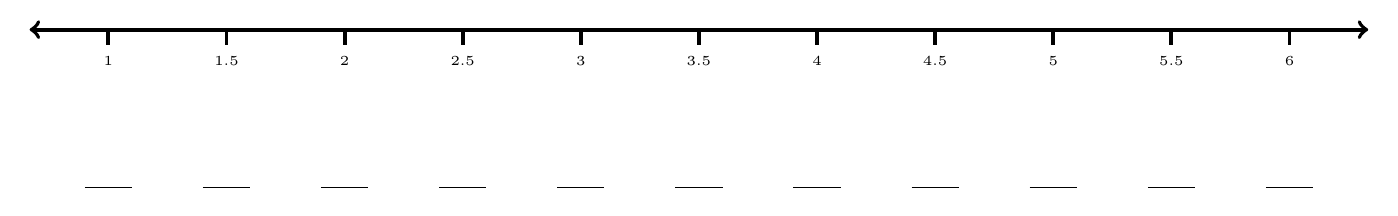
\begin{tikzpicture}
\draw[black, line width=0.5mm, <->](-1,0)--(16,0);
\foreach \x in {1,1.5,...,6}{
\draw[black, line width=0.5mm](3*\x-3,0)--(3*\x-3,-0.2)node[below]{\tiny \x };
\draw[black, line width=0.1mm](3*\x-3.3,-2)--(3*\x-2.7,-2);
}
\end{tikzpicture}
\end{center}
\vspace{1cm}
For each number, write it as a square root below it. For example, below the number 3, write $\sqrt{9}$ and below 2.5 write $\sqrt{6.25}$.\\\\
Using arrows identify approximately where $\sqrt{2}$ , $\sqrt{3}$, $\sqrt{5}$, $\sqrt{10}$, $\sqrt{12}$ would be.\\

\subsection{Cube Roots}
The cube root of a number is another number that multiplied by itself 3 times is equal to that number.\\\\
For example:    $4\times4\times4=64$         so 4 is the cube root of 64\\
The sign for a cube root is: $\sqrt[3]{~~~}$\\\\
We can also have symbols such as $\sqrt[4]{~~~}$, $\sqrt[5]{~~~}$\\\\
\textbf{Find}
\begin{enumerate*}
	\item ~~$\sqrt[3]{8}=$~~~~~~~~~~~~~~~
	\item ~~$\sqrt[3]{27}=$~~~~~~~~~~~~~~~
	\item ~~$\sqrt[3]{343}=$~~~~~~~~~~~~~~~
\end{enumerate*}\\\\
\textbf{List:} all the perfect squares cubic numbers 1 to 200.\\\\
\textbf{Question:} what is $\sqrt[3]{-8}$? \\
Can we have cube roots of negative numbers? (what about square roots?).
\newpage
\subsection {Working with Surds}
The types of numbers that we have dealt with are called \textbf{Surds}. The word is actually related to the word "absurd" because absurd means irrational!\\\\
By looking at some individual cases, we can work out some rules for working with surds.\\
Using your calculators work out the following (round to 4dp):
\begin{enumerate}
	\item -
	\begin{enumerate}
		\item $\sqrt{3}\times\sqrt{6}=$
		\item $\sqrt{3\times6}=$
	\end{enumerate}
	\item -
	\begin{enumerate}
		\item $\sqrt{2}\times\sqrt{8}=$
		\item $\sqrt{2\times8}=$
	\end{enumerate}
\end{enumerate}
From this we can establish a rule for Surds:
\begin{equation*}
\begin{split}
\sqrt{a}\times\sqrt{b}&=\sqrt{ab}\\
\text{and~~~~~~~~~~~~~~~}\sqrt{ab}&=\sqrt{a}\times\sqrt{b}\\
\end{split}
\end{equation*}\\
The second statement allows us to put all of a mutiplication under a square root:\\\\
For example:\\\\
 $3\times\sqrt{2}=\sqrt{9}\times\sqrt{2}=\sqrt{18}$.\\\\
 $4\times\sqrt{7}=\sqrt{16}\times\sqrt{7}=\sqrt{112}$.
\\\\
This knowledge also allows us to "clean up" square roots by having the simplest possible value underneath the square root and the rest outside as a multiplier.\\\\
This know as putting the square root in the form:~~ $a\sqrt{b}$\\
\newpage
\subsubsection{Exercises (Working with Surds)}
\begin{enumerate}
	\item Write these surds underneath a single square root. Evaluate them if they make a perfect square otherwise, leave them in surd form.
	\begin{multicols}{2}
		\begin{enumerate}
			\item $\displaystyle \sqrt{3}\times \sqrt{7}= $
			\item $\displaystyle \sqrt{5}\times \sqrt{6}= $
			\item $\displaystyle \sqrt{5}\times \sqrt{20}=$
			\item $\displaystyle \sqrt{3}\times \sqrt{12}=$
			\item $\displaystyle \sqrt{6}\times \sqrt{24}=$
			\item $\displaystyle \sqrt{3}\times \sqrt{27}=$		
		\end{enumerate}
	\end{multicols}
	\item By writing the number outside the square root in square root form, write these expressions underneath a single square root.
	\begin{multicols}{2}
		\begin{enumerate}
			\item $\displaystyle 5\times \sqrt{2}= $
			\item $\displaystyle 7\times \sqrt{2}= $
			\item $\displaystyle 3\times \sqrt{5}=$
			\item $\displaystyle 4\times \sqrt{3}=$
			\item $\displaystyle 5\times \sqrt{5}=$
			\item $\displaystyle 11\times \sqrt{27}=$		
		\end{enumerate}
	\end{multicols}
	\begin{align*}
	\text{If we write}&& 2\sqrt{7}&\\
	\text{This means}&& 2\times \sqrt{7}&\\
	\text{Consequently}&& 4\sqrt{7}\times 3\sqrt{6}&=4\times \sqrt{7}\times 3\times \sqrt{6}\\
	&&&=12\times \sqrt{7} \times \sqrt{6}\\
	&&&=12\sqrt{42}
	\end{align*}
	\item Write the following in the form $a\sqrt{b}$.
	(\footnotesize For example: $2\sqrt{7}\times 3\sqrt{4}=6\sqrt{28}$ \normalsize)
	\begin{multicols}{2}
		\begin{enumerate}
			\item $\displaystyle 2\sqrt{7}\times 4\sqrt{3}=$
			\item $\displaystyle 2\sqrt{8}\times 5\sqrt{5}=$
			\item $\displaystyle 2\sqrt{32}\times 3\sqrt{2}=$
			\item $\displaystyle 5\sqrt{3}\times 4\sqrt{21}=$
			\item $\displaystyle 4\sqrt{18}\times 2\sqrt{5}=$
			\item $\displaystyle 2\sqrt{6}\times 5\sqrt{42}=$
		\end{enumerate}
	\end{multicols}
	\begin{align*}
	\text{Working the other way:}&\\
	\text{If we have a surd such as~~} \sqrt{32}&\\
	\text{If we can find \textbf{a square number that is a factor},we can write~~} \sqrt{32}&=\sqrt{16\times 2}\\
	&=\sqrt{16}\times \sqrt{2}\\
	&=4\sqrt{2} 
	\end{align*}
	\item Find square number factors for the following and write the surds in the form $a\sqrt{b}$
	\begin{multicols}{2}
		\begin{enumerate}
			\item $\displaystyle \sqrt{8}=$
			\item $\displaystyle \sqrt{27}=$
			\item $\displaystyle \sqrt{80}=$
			\item $\displaystyle \sqrt{108}=$
			\item $\displaystyle \sqrt{405}=$
			\item $\displaystyle \sqrt{112}=$
			\item $\displaystyle \sqrt{63}=$
			\item $\displaystyle \sqrt{180}=$
		\end{enumerate}
	\end{multicols}
\end{enumerate}
\newpage






\section{Practice Questions}
\subsection{Practice Questions 1}
\newcommand{\wdth}{2}
\newcommand{\hght}{1}
\begin{enumerate}
	\item Definitions
	\begin{enumerate}
		\item What is the definition of a \textbf{factor}?
		\item What is the definition of a \textbf{multiple}?
		\item What is the definition of a \textbf{prime number}?
	\end{enumerate}
	\item In each set of Whole Numbers, circle the prime numbers.\\
	(remember that the division test numbers will be 2,3,5,7).
	\begin{enumerate}
		\item \{40, 41, 42, 43, 44, 45, 46, 47, 48, 49\}
		\item \{65, 66, 67, 68, 69, 70, 71, 72, 73, 74\}
		\item \{83, 84, 85, 86, 87, 88, 89, 90, 91, 92\}
	\end{enumerate} 
	\item Make factor trees for the following numbers (unless the number is prime) and write each number as a product of its prime factors.
	\begin{multicols}{4}
		\begin{enumerate}
			\item 100
			\item 120
			\item 164
			\item 163
		\end{enumerate}
	\end{multicols}
	\item Find the Lowest Commmon Multiple for the following pairs of prime numbers
	\begin{multicols}{5}
		\begin{enumerate}
			\item 12, 26
			\item 18, 33
			\item 52, 169
			\item 56, 108
			\item 84, 96
		\end{enumerate}
	\end{multicols}
	\item Write factor lists for:
	\begin{multicols}{4}
		\begin{enumerate}
			\item 144
			\item 196
			\item 220
			\item 180
		\end{enumerate} 
	\end{multicols}
	\item Calculate the following
	\begin{multicols}{3}
		\begin{enumerate}
			\item $\displaystyle -17-21= $
			\item $\displaystyle -26--14= $
			\item $\displaystyle -105+-3$
			\item $\displaystyle -17\times -3=$
			\item $\displaystyle 15\div -3=$
			\item $\displaystyle 4\times -8=$
		\end{enumerate}
	\end{multicols}
	\item The two bricks below add to the brick above. Fill in the missing bricks:\\
	\begin{center}
		\begin{tikzpicture}
		\draw[black, thin] (0,0) rectangle (\wdth,\hght)node[midway]{$-5$};
		\draw[black, thin] (\wdth,0) rectangle (2*\wdth,\hght);
		\draw[black, thin] (2*\wdth,0) rectangle (3*\wdth,\hght)node[midway]{$-7$};
		\draw[black, thin] (\wdth/2,\hght) rectangle (3*\wdth/2,2*\hght)node[midway]{$6$};
		\draw[black, thin] (3*\wdth/2,\hght) rectangle (5*\wdth/2,2*\hght);
		\draw[black, thin] (\wdth,2*\hght) rectangle (2*\wdth,3*\hght);
		\end{tikzpicture}
	\end{center}
	\newpage
	\item The numbers in the circles \textbf{multiply} to give the number in the squares between them. Fill in the missing spaces:\\
	\begin{center}
		\begin{tikzpicture}
		\coordinate (A) at (0,0);
		\coordinate (B) at (3*\wdth,0);
		\coordinate (C) at (1.5*\wdth,4*\hght);
		\draw[black, thin] (A)--(B)--(C)--(A);
		\filldraw[draw=black,fill=white, thin] (A) circle[radius=0.6cm]node{$-3$};
		\filldraw[draw=black,fill=white, thin] (B) circle[radius=0.6cm]node{$-8$};
		\filldraw[draw=black,fill=white, thin] (C) circle[radius=0.6cm];
		\filldraw[draw=black,fill=white, thin] (0.75*\wdth-0.5,2*\hght-0.5) rectangle(0.75*\wdth+0.5,2*\hght+0.5)node[midway]{$15$};
		\filldraw[draw=black, fill=white, thin] (2.25*\wdth-0.5,2*\hght-0.5) rectangle(2.25*\wdth+0.5,2*\hght+0.5);
		\filldraw[draw=black,fill=white, thin] (1.5*\wdth-0.5,0-0.5) rectangle(1.5*\wdth+0.5,0+0.5);
		\end{tikzpicture}
	\end{center}
	\item (Difficult)Calculate the following
	\begin{multicols}{3}
		\begin{enumerate}
			\item $\displaystyle (-3)^{2}\div 9= $
			\item $\displaystyle -3\times (-4)\div \sqrt{36}= $
			\item $\displaystyle -16\div -2\times (5+-7)=$
			\item $\displaystyle (-2^{5}+3)\times -7=$
			\item $\displaystyle (-2+3)^{20}\times \sqrt[3]{27}=$
			\item $\displaystyle 4^{4}\times -0.5+\sqrt{121}=$
		\end{enumerate}
	\end{multicols}
	\item Write the following Decimals as Fractions
	\begin{multicols}{4}
		\begin{enumerate}
			\item $\displaystyle 0.\dot{3}$
			\item $\displaystyle 0.\dot{6}$
			\item $\displaystyle 0.\dot{4}$
			\item $\displaystyle 0.\dot{8}$
		\end{enumerate}
	\end{multicols}
	\item Write the following Decimals as Fractions
	\begin{multicols}{4}
		\begin{enumerate}
			\item $\displaystyle 0.\dot{3}\dot{5}$
			\item $\displaystyle 0.\dot{6}\dot{8}$
			\item $\displaystyle 0.\dot{4}\dot{1}$
			\item $\displaystyle 0.\dot{8}\dot{1}$
		\end{enumerate}
	\end{multicols}
	\item (Difficult)Write the following Decimals as Fractions
	\begin{multicols}{4}
		\begin{enumerate}
			\item $\displaystyle 0.7\dot{5}$
			\item $\displaystyle 0.1\dot{8}$
			\item $\displaystyle 0.1\dot{6}$
			\item $\displaystyle 0.9\dot{8}$
		\end{enumerate}
	\end{multicols}
	\item Evaluate the following:
	\begin{multicols}{4}
		\begin{enumerate}
			\item $\displaystyle 9^{2}-\sqrt{900}$
			\item $\displaystyle (-2)^{9}$
			\item $\displaystyle 121^{\frac{1}{2}}$
			\item $\displaystyle 5^{-3}$
		\end{enumerate}
	\end{multicols}
	\item Simplify:
	\begin{multicols}{4}
		\begin{enumerate}
			\item $\displaystyle \sqrt{7}\times \sqrt{12}$
			\item $\displaystyle \sqrt{12}\times \sqrt{3}$
			\item $\displaystyle \sqrt{0.5}\times \sqrt{2}$
			\item $\displaystyle \frac{4}{\sqrt{32}}\times \frac{4}{\sqrt{2}}$
		\end{enumerate}
	\end{multicols}
	\item Write the following surds in the form $\displaystyle a\sqrt{b}$:
	\begin{multicols}{4}
		\begin{enumerate}
			\item $\displaystyle  \sqrt{360}$
			\item $\displaystyle \sqrt{50}$
			\item $\displaystyle \sqrt{216}$
			\item $\displaystyle \sqrt{500}$
		\end{enumerate}
	\end{multicols}
\end{enumerate}
\newpage
\section{Extension Practice}
\begin{enumerate}
	\item Find the Highest Common Factor of 504 and 162
	\item Find the Lowest Common Multiple of 882 and 336
	\item Identify the Prime Numbers in the set \{130, 131, 132, 133, 134, 135, 136, 137, 138, 139\}.
	\item A shop is running a special on chocolate bars and is selling them at a price between 50c and \$1. Johnny pays \$9.24 for the ones he buys, while Jessica pays \$5.88 for hers.\\
	What is the price of a chocolate bar and how many more did Johnny buy than Jessica?
	\item Calculate
	\begin{enumerate}
		\item $\displaystyle [(-3)^{2}+4]^{2}+-3\times -8=$
		\item $\displaystyle -3^{2}-4\div2-(-4)^{2}=$
		\item $\displaystyle [-(14-17)]^{3}\times -2^{7}=$
		\item $\displaystyle 2\div 4\div \frac{1}{2}\div \sqrt{0.25}=$
	\end{enumerate}
	\item Convert the following decimals to fractions.
	\begin{enumerate}
		\item $\displaystyle 0.1\dot{8}$
		\item $\displaystyle 0.\dot{2}34\dot{7}$
		\item $\displaystyle 0.25\dot{1}$
	\end{enumerate}
	\item Write the following surds with a rational number as the denominator
	\begin{enumerate}
		\item $\displaystyle \frac{\sqrt{7}}{\sqrt{8}}$
		\item $\displaystyle \frac{1}{\sqrt{2}}$
		\item $\displaystyle \frac{\sqrt{3}}{\sqrt{5}+\sqrt{8}}$
	\end{enumerate}
	
	
\end{enumerate}


\newpage
\section{Answers}
\footnotesize
\ref{factorlists}
\begin{multicols}{4}
	\begin{enumerate}[label= \roman*)]
		\item 1,24 ; 2,12 ; 3,8 ; 4,6 
		\item 1,30 ; 2,15 ; 3, 10 ; 5,6 
		\item 1,48 ; 2,24 ; 3,16 ; 4,12 ; 6,8
		\item 1,84 ; 2,42 ; 3,28 ; 4,21 ; 6,14 ; 7,12  
		\item 1,96 ; 2,48 ; 3,32 ; 4,24 ; 6,16 ; 8,12
		\item 1,221 ; 13,17   
		\item 1,210 ; 2,105 ; 3,70 ; 5,42 ; 6,35 ; 7,30 ; 10,21 ; 14,15
	\end{enumerate}
\end{multicols}
\ref{factortrees}
\begin{multicols}{4}
	\begin{enumerate}[label= \roman*)]
		\item $2\times2\times2\times3=24$
		\item $2\time3\times5=30$ 
		\item $2\time2\times2\times2\times3=48$
		\item $2\time2\times3\times7=84$  
		\item $2\time2\times2\times2\times2\times2\times3=96$
		\item $13\times17=221$   
		\item $2\times3\times5\times7=210$
	\end{enumerate}
\end{multicols}
\ref{hcf1}
\begin{multicols}{4}
	\begin{enumerate}[label= \roman*)]
		\item $HCF(48,54)=6$
		\item $HCF(96,120)=24$ 
		\item $HCF(64,32)=32$
		\item $HCF(120,160)=40$  
	\end{enumerate}
\end{multicols}
\ref{hcfVenn}
\begin{multicols}{4}
	\begin{enumerate}[label= \roman*)]
		\item $HCF(32,48)=16$
		\item $HCF(48,54)=6$ 
		\item $HCF(64,84)=4$
		\item $HCF(72,96)=24$  
	\end{enumerate}
\end{multicols}
\ref{LCM}
\begin{multicols}{5}
	\begin{enumerate}[label= \roman*)]
		\item $LCM(15,10)=30$
		\item $LCM(20,24)=120$ 
		\item $LCM(16,28)=112$
		\item $LCM(14,21)=42$  
		\item $LCM(19,6)=114$
	\end{enumerate}
\end{multicols}
\ref{LCMVenn}
\begin{multicols}{4}
	\begin{enumerate}[label= \roman*)]
		\item $LCM(12,18)=36$
		\item $LCM(32,52)=416$ 
		\item $LCM(64,100)=1600$
		\item $LCM(210,200)=4200$  
	\end{enumerate}
\end{multicols}
\ref{SetOne}
\begin{enumerate}
	\item 
	\begin{enumerate}
		\item 8
		\item 9
		\item 24
		\item 12
	\end{enumerate}
	\item
	\begin{enumerate}
		\item  A=269,724 ; B=1,379,724 ; HCF(A,B)=10,374
	\end{enumerate}
	\item
	\begin{enumerate}
		\item A=66,300 ; B=10,710 ; HCF(A,B)=510
		\item A=33,700,290 ; B=234,600 ; HCF(A,B)=11,730
	\end{enumerate}
	\item A=4410 ; B=168 ; C=420
	\begin{enumerate}
		\item  HCF(A,B,C)=42?
		\item  LCM(A,B,C)17,640?
	\end{enumerate}
\end{enumerate}
\ref{SetTwo}
\begin{enumerate}
	\item C. 6 packages of pencils and 5 packages of erasers.
	\item HCF(30,48)=6 , 6 Containers (5 oat and 8 choc chip)
	\item 
	\begin{enumerate}
		\item LCM(12,18)=36   (36 cm)
		\item 36cm ,72cm, 108cm,...
	\end{enumerate}
\end{enumerate}
\ref{SetThree}
\begin{enumerate}
	\item D. Every 60 minutes
	\item A factor of a number divides completely into the number, a multiple of a number is any whole number times the number
	\item LCM(4,6)=12 ; Flashes together 0,12,24,36,48,60 (6 times)
	\item LCM(5,3)=15 ; May 20th
	\item A: 16
	\item LCM(2,7,10)=LCM(LCM(2,7),10)=LCM(14,10)= 70; Every 70th Visitor
	\item LCM(8,12)=24 ; 3 x hot dog packages , 2 x hot dog buns
\end{enumerate}
\ref{SetFour}
\begin{enumerate}
	\item LCM(5,7)=35; In 35 days jack paints 7 houses, and Jill paints 5 houses.\\
	12 houses in 35 days ; 1 house in $\frac{35}{12}$ days. \\
	$2 \frac{11}{12}$ days.
	\item LCM(3,5,6)=30; In 30 hours Bill can load 10 trucks, Jane 6 trucks and Jonny 5 trucks.\\
	They can load 21 trucks in 30 hours, so can load one truck in $\frac{30}{21}$ hours\\
	$1\frac{3}{7}$ hour.
	\item LCM(12,10)=60 ; In 60 minutes the ferries will complete 5 + 6 = 11 trips.\\
	They will have covered one total trip in $\frac{60}{11}$ minutes.\\
	$5\frac{5}{11}$ minutes
	\item LCM(52,48)=624 ; in 624 seconds A does 12 x 400 and B does 13 x 400.\\
	25 x 400 in 624 seconds.\\
	1 x 400 in $\frac{624}{25}$ seconds\\
	$24\frac{24}{25}$ seconds.
	\item LCM(8,10)=40 ; 9 baths filled in 40 minutes ; 1 bath in $\frac{40}{9}$ minutes.
	\item Pat completes $\frac{9}{15}$ of the job in 9 hours, so Andy has completed $\frac{6}{15}$ of the job in 9 hours ; so Andy can complete the whole job in $\frac{15}{6}\times 9 = 22\frac{1}{2}$ hours.
	\item LCM(12,16)=48 ; 7 full journeys completed in 48 hours ; 1 full journey in $\frac{48}{7}=6\frac{6}{7}$ hours
	\item The other train does $\frac{2}{5}$ of a journey in 3 hours so the other train takes $\frac{5}{2}\times 3 =\frac{15}{2}= 7\frac{1}{2}$ hours to complete the journey.
\end{enumerate}
\ref{submalloon}
\begin{figure}[!h]
	\centering
	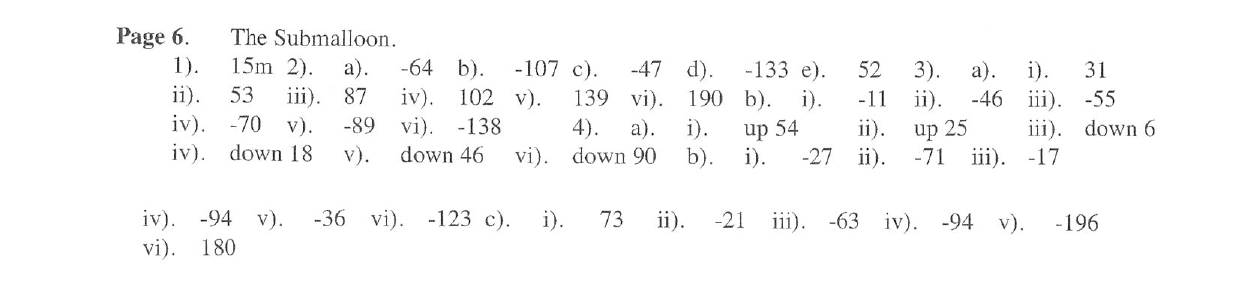
\includegraphics[width=18cm]{Submalloon_solutions}
	% \caption{a nice plot}
	%\label{fig:mesh1}
\end{figure}\\
\ref{IntOne}
	\begin{multicols}{3}
		\begin{enumerate}[label=\footnotesize \roman*)]
			\item~~~$3+5=8$
			\item~~~$3-5=-2$
			\item~~~$2+8=10$
			\item~~~$2-8=-6$
			\item~~~$1+12=13$
			\item~~~$1-12=-11$
			\item~~~$4+9=13$
			\item~~~$4-9=-5$
			\item~~~$7+14=21$
			\item~~~$7-14=-7$
			\item~~~$18+27=45$
			\item~~~$18-27=-9$
		\end{enumerate}
	\end{multicols}
\ref{IntTwo}
	\begin{multicols}{3}
		\begin{enumerate}[label=\footnotesize \roman*)]
			\item~~~$-3+5=2$
			\item~~~$-3-5=-8$
			\item~~~$-2+8=6$
			\item~~~$-2-8=-10$
			\item~~~$-1+12=11$
			\item~~~$-1-12=-13$
			\item~~~$-4+9=5$
			\item~~~$-4-9=-13$
			\item~~~$-7+14=7$
			\item~~~$-7-14=-21$
			\item~~~$-18+13=-5$
			\item~~~$-18-32=-50$
		\end{enumerate}
	\end{multicols}
\ref{IntThree}
	\begin{multicols}{3}
		\begin{enumerate}[label=\footnotesize \roman*)]
			\item~~~$-13+5=-8$
			\item~~~$9-12=-3$
			\item~~~$-2+1=-1$
			\item~~~$-2+0=-2$
			\item~~~$-15+6=-9$
			\item~~~$-18-30=-48$
			\item~~~$-21+24=3$
			\item~~~$-70-9=-79$
			\item~~~$-70+9=-61$
			\item~~~$-70-24=-94$
			\item~~~$-70+24=-46$
			\item~~~$-70+104=34$
		\end{enumerate}
	\end{multicols}
\ref{IntFour}
	\begin{multicols}{3}
		\begin{enumerate}[label=\footnotesize \roman*)]
			\item~~~$3+5=8$
			\item~~~$3-5=-2$
			\item~~~$3+-5=-2$
			\item~~~$3--5=8$
			\item~~~$1+12=13$
			\item~~~$1-12=-11$
			\item~~~$1+-12=-11$
			\item~~~$1--12=13$
			\item~~~$7+14=21$
			\item~~~$7-14=-7$
			\item~~~$7+-14=-7$
			\item~~~$7--14=21$
		\end{enumerate}
	\end{multicols}
\ref{IntFive}


	\begin{multicols}{3}
		\begin{enumerate}[label=\footnotesize \roman*)]
			\item~~~$-3+5=2$
			\item~~~$-3-5=-8$
			\item~~~$-3+-5=-8$
			\item~~~$-3--5=2$
			\item~~~$-10-6=-16$
			\item~~~$-10+6=-4$
			\item~~~$-10--6=-4$
			\item~~~$-10+-6=-16$
			\item~~~$-7--14=7$
			\item~~~$-7+14=7$
			\item~~~$-7-14=-21$
			\item~~~$-7+-14=-21$
		\end{enumerate}
	\end{multicols}
\ref{IntSix}
	\begin{multicols}{3}
		\begin{enumerate}[label=\footnotesize \roman*)]
			\item~~~$-12+5=-7$
			\item~~~$ 16-5=11$
			\item~~~$23+-15=8$
			\item~~~$30--25=55$
			\item~~~$-10--6=-4$
			\item~~~$22+-30=-8$
			\item~~~$-45--10=-35$
			\item~~~$-21-6=-27$
			\item~~~$-19+-14=-33$
			\item~~~$-70+14=-56$
			\item~~~$-9-14=-23$
			\item~~~$-1--14=13$
		\end{enumerate}
	\end{multicols}
\ref{IntSeven}
	\begin{multicols}{3}
		\begin{enumerate}[label=\footnotesize \roman*)]
			\item~~~$5+A=15$; A=10
			\item~~~$ A-5=-2$; A=3
			\item~~~$15+A=-6$; A=-21
			\item~~~$A--6=13$; A=7
			\item~~~$0-A=-8$; A =8
			\item~~~$0+A=-8$; A=-8
			\item~~~$-15--A=1$; A=16
			\item~~~$-8-A=90$; A=-98
			\item~~~$-19+2\times A=-3$; A=8
			\item~~~$-A+14=-15$; A=29
			\item~~~$A-14=-120$; A=-106
			\item~~~$A--14=-25$; A=-39
		\end{enumerate}
	\end{multicols}
\ref{pyramids}
\begin{multicols}{3}
	\boxesSols{17}{2}{15}{-7}{9}{6}{1}
	\boxesSols{10}{12}{-2}{4}{8}{-10}{4}
	\boxesSols{-2}{-4}{2}{1}{-5}{7}{2}
	\boxesSols{-44}{-20}{-24}{-9}{-11}{13}{5}
	\boxesSols{-12}{-8}{-4}{-15}{7}{-11}{3}
	\boxesSols{-29}{-8}{-21}{7}{-15}{-6}{6}
\end{multicols}
\newpage
\begin{multicols}{3}
	\boxesSols{6}{9}{-3}{5}{4}{-7}{7}
	\boxesSols{-9}{-10}{1}{-7}{-3}{4}{10}
	\boxesSols{3}{9}{-6}{6}{3}{-9}{8}
	\boxesSols{-6}{-1}{-5}{-5}{4}{-9}{11}
	\boxesSols{-1}{-7}{6}{-9}{2}{4}{9}
	\boxesSols{-24}{-3}{-21}{12}{-15}{-6}{12}
\end{multicols}
\begin{multicols}{3}
	\boxesSols{3}{-3}{6}{-7}{4}{2}{13}
	\vfill\null
	\columnbreak
	\boxesSols{-9}{-17}{8}{-11}{-6}{14}{14}
	\vfill\null
	\columnbreak
	\boxesSols{-2}{0}{-2}{-8}{8}{-10}{15}
\end{multicols}
\ref{magicsquares}
\begin{multicols}{3}
	\magicsquareASols{0,7,2,5,3,1,4,-1,6,1,9}
	\magicsquareASols{1,2,6,8,3,-2,0,4,5,4,9}
	\magicsquareASols{0,-1,4,5,1,-3,-2,3,2,2,3}
	\magicsquareASols{3,-3,6,5,2,-1,-2,7,1,5,6}
	\magicsquareASols{-4,3,-2,1,-1,-3,0,-5,2,3,-3}
	\magicsquareASols{4,-4,3,0,1,2,-1,6,-2,6,3}
\end{multicols}\vspace{-0.5cm}
\begin{multicols}{3}
	\magicsquareASols{-6,-1,-8,-7,-5,-3,-2,-9,-4,7,-15}
	\magicsquareASols{-2,-8,1,0,-3,-6,-7,2,-4,10,-9}
	\magicsquareASols{-8,-2,-11,-10,-7,-4,-3,-12,-6,8,-21}
	\magicsquareASols{-5,-6,-1,0,-4,-8,-7,-2,-3,11,-12}
	\magicsquareASols{-5,-12,-7,-10,-8,-6,-9,-4,-11,9,-24}
	\magicsquareASols{3,-2,5,4,2,0,-1,6,1,12,6}
\end{multicols}

\ref{multInt0}
	\begin{multicols}{3}
	\begin{enumerate}[label=\footnotesize \roman*)]
		\item~~~$3\times2=6$
		\item~~~$3\times-2=-6$
		\item~~~$-3\times2=-6$
		\item~~~$-3\times-2=6$
		\item~~~$-7\times-8=56$
		\item~~~$-7\times8=-56$
		\item~~~$7\times-8=-56$
		\item~~~$7\times8=56$
		\item~~~$-9\times12=-108$
		\item~~~$-3\times9=-27$
		\item~~~$4\times-8=-32$
		\item~~~$-7\times-9=63$
	\end{enumerate}
\end{multicols}
\ref{multInt1}
	\begin{multicols}{3}
	\begin{enumerate}[label=\footnotesize \roman*)]
		\item~~~$-15\times3=-45$
		\item~~~$5\times15=75$
		\item~~~$4\times-15=-60$
		\item~~~$-2\times-16=32$
		\item~~~$-16\times -3=48$
		\item~~~$4\times16=64$
		\item~~~$2\times-24=-48$
		\item~~~$8\times-20=-160$
		\item~~~$-25\times6=-150$
		\item~~~$-35\times3=-105$
		\item~~~$-13\times-3=39$
		\item~~~$-14\times3=-42$
	\end{enumerate}
\end{multicols}
\ref{multInt2}
	\begin{multicols}{3}
	\begin{enumerate}[label=\footnotesize \roman*)]
		\item~~~$-36\div3=-12$
		\item~~~$45\div-9=-5$
		\item~~~$-54\div6=-9$
		\item~~~$-16\div-2=8$
		\item~~~$96\div12=8$
		\item~~~$-96\div-32=3$
		\item~~~$96\div-24=-4$
		\item~~~$96\div-16=-6$
		\item~~~$-121\div11=-11$
		\item~~~$-75\div-15=5$
		\item~~~$-169\div-13=13$
		\item~~~$225\div-5=-45$
	\end{enumerate}
\end{multicols}
\ref{multInt3}
	\begin{multicols}{3}
	\begin{enumerate}[label=\footnotesize \roman*)]
		\item~~~$\displaystyle \frac{-36}{-3}=12$
		\item~~~$\displaystyle \frac{36}{-3}=-12$
		\item~~~$\displaystyle \frac{-18}{-9}=2$
		\item~~~$\displaystyle \frac{-45}{15}=-3$
		\item~~~$\displaystyle \frac{64}{16}=4$
		\item~~~$\displaystyle \frac{56}{-8}=-7$
		\item~~~$\displaystyle \frac{-72}{-9}=8$
		\item~~~$\displaystyle \frac{72}{24}=3$
		\item~~~$\displaystyle \frac{84}{-12}=-7$
		\item~~~$\displaystyle \frac{-84}{-6}=14$
		\item~~~$\displaystyle \frac{-105}{-5}=21$
		\item~~~$\displaystyle \frac{-125}{25}=-5$
	\end{enumerate}
\end{multicols}
\ref{multInt4}
	\begin{multicols}{3}
	\begin{enumerate}[label=\footnotesize \roman*)]
		\item~~~$-8\times B=48; B=-6$
		\item~~~$B\times12=84; B=7$
		\item~~~$B\times-3=-21; B=7$
		\item~~~$-B\times-3=21; B=-7$
		\item~~~$-16\times B=-48; B=3$
		\item~~~$2\times B \times-6=48; B=-4$
		\item~~~$-3\times B \times -7=63; B=3$
		\item~~~$B \times-20 \times -3=-180; B=-3$
		\item~~~$-B\times -7=91; B=13$
		\item~~~$B\times3=-90; B=-30$
		\item~~~$17\times B= -51; B=-3$
		\item~~~$-16\times B=48; B=-3$
	\end{enumerate}
\end{multicols}
\ref{multInt5}
\begin{multicols}{3}
	\begin{enumerate}[label=\footnotesize \roman*)]
		\item~~~$\displaystyle \frac{D}{-2}=-12; D=24$
		\item~~~$\displaystyle \frac{D}{-3}=5; D=-15$
		\item~~~$\displaystyle \frac{-D}{-9}=3; D=27$
		\item~~~$\displaystyle \frac{-D}{15}=2; D=-30$
		\item~~~$\displaystyle \frac{12}{D}=3; D=4$
		\item~~~$\displaystyle \frac{35}{D}=7; D=5$
		\item~~~$\displaystyle \frac{-45}{D}=9; D=-5$
		\item~~~$\displaystyle \frac{-99}{D}=-11; D=9$
		\item~~~$\displaystyle \frac{78}{D}=39; D=2$
		\item~~~$\displaystyle \frac{-78}{D}=13; D=-6$
		\item~~~$\displaystyle \frac{-5\times D}{2}=10; D=-4$
		\item~~~$\displaystyle \frac{4 \times D -5}{25}= -1; D=-5$
	\end{enumerate}
\end{multicols}
\ref{exp0}
\begin{multicols}{3}
	\begin{enumerate}
		\item ~~~~$7^{2}=49$
		\item ~~~~$4^{3}=64$
		\item ~~~~$2^{4}=16$
		\item ~~~~$5^{3}=125$
		\item ~~~~$\displaystyle \Big(\frac{1}{3}\Big)^{2}=\frac{1}{9}$
		\item ~~~~$\displaystyle \Big(\frac{1}{3}\Big)^{4}=\frac{1}{81}$
		\item ~~~~$\displaystyle \Big(\frac{1}{5}\Big)^{3}=\frac{1}{125}$
		\item ~~~~$\displaystyle \Big(\frac{1}{2}\Big)^{5}=\frac{1}{32}$
	\end{enumerate}
\end{multicols}
\ref{exp1}
	\begin{multicols}{3}
	\begin{enumerate}[label=\footnotesize \roman*)]
		\item~~~$\displaystyle 2^5=32$
		\item~~~$\displaystyle 3^2=9$
		\item~~~$\displaystyle -3^2=-9$
		\item~~~$\displaystyle (-3)^2=9$
		\item~~~$\displaystyle 4^3=64$
		\item~~~$\displaystyle (-4)^3=-64$
		\item~~~$\displaystyle 5^2=25$
		\item~~~$\displaystyle (-5)^3=-125$
		\item~~~$\displaystyle 6^2=36$
		\item~~~$\displaystyle 7^3=343$
		\item~~~$\displaystyle \Big(\frac{1}{2}\Big)^{5}=\frac{1}{32}$
		\item~~~$\displaystyle \Big(\frac{2}{3}\Big)^{3}=\frac{8}{27}$
	\end{enumerate}
\end{multicols}
\ref{exp2}
\begin{multicols}{3}
	\begin{enumerate}[label=\footnotesize \roman*)]
		\item~~~$\displaystyle 3^P=27;~~P=3$
		\item~~~$\displaystyle 4^P=64;~~P=3$
		\item~~~$\displaystyle 5^P=625;~~P=4$
		\item~~~$\displaystyle 10^P=1000;~~P=3$
		\item~~~$\displaystyle 10^P=1000000;~~P=6$
		\item~~~$\displaystyle 2^P=4^3;~~P=6$
		\item~~~$\displaystyle 3^{2 \times P}=81;~~P=2$
		\item~~~$\displaystyle 5^{3 \times P}=125;~~P=1$
		\item~~~$\displaystyle 7^{P-8}=343;~~P=11$
	\end{enumerate}
\end{multicols}
\ref{op1}
	\begin{multicols}{2}
	\begin{enumerate}[label=\footnotesize \roman*)]
		\item ~~~~$2^3+8-20=-4$
		\item ~~~~$3^{2}-10=-1$
		\item ~~~~$2\times3^2=18$
		\item ~~~~$4\times3^3=108$
		\item ~~~~$0\times4^{21}=0$
		\item ~~~~$4\times(2^3-6)=8$
		\item ~~~~$3\times(5-6)=-3$
		\item ~~~~$-3\times(5+8)=-39$
		\item ~~~~$-3\times(8-5)=-9$
		\item ~~~~$3\times(8-5)\times(4+3)=63$
	\end{enumerate}
\end{multicols}
\ref{op2}
	\begin{multicols}{2}
	\begin{enumerate}[label=\footnotesize \roman*)]
		\item ~~~~$-3+4\div-2+7=2$
		\item ~~~~$-3\times4+-6\div2=-15$
		\item ~~~~$-14+-2\times-3=-8$
		\item ~~~~$15+-4--3\times3=20$
		\item ~~~~$(13--1)\times11-1=153$
		\item ~~~~$11--7\times3+12=44$
		\item ~~~~$11--7\times3\times-4=-73$
		\item ~~~~$-3\times2--8=2$
		\item ~~~~$-11+4\div-1=-15$
		\item ~~~~$121--4\times-1\times-6=145$
		\item ~~~~$12--4\times7+6\times-9=-14$
		\item ~~~~$-12--12--1-1=-2$
		\item ~~~~$12\times(1--5)\times-1+11=-61$
		\item ~~~~$(2-5)\times(3+8)\div-3=11$
		\item ~~~~$(-12\times(2+3)+11)\times(6\div3)=-98$
		\item ~~~~$(3\times(4-13)+7)\times5=-100$
	\end{enumerate}
\end{multicols}
\ref{Dec1}
\begin{multicols}{2}
	\begin{enumerate}
		\item ~~~~$\displaystyle 0.35=\frac{35}{100}=\frac{7}{20}$
		\item ~~~~$\displaystyle 0.675=\frac{675}{1000}=\frac{27}{40}$
		\item ~~~~$\displaystyle 0.625=\frac{625}{1000}=\frac{5}{8}$
		\item ~~~~$\displaystyle 0.42=\frac{42}{100}=\frac{21}{50}$
		\item ~~~~$\displaystyle 0.212=\frac{212}{1000}=\frac{53}{250}$
		\item ~~~~$\displaystyle 0.0308=\frac{0308}{10000}=\frac{77}{2500}$
		\item ~~~~$\displaystyle 0.10608=\frac{10608}{100000}=\frac{663}{6250}$
		\item ~~~~$\displaystyle 0.3042=\frac{3042}{10000}=\frac{1521}{5000}$
	\end{enumerate}
\end{multicols}
\ref{Dec2}
		\begin{multicols}{3}
	\begin{enumerate}
		\item 
		\begin{enumerate}
			\item $\displaystyle 0.\dot{2}=\frac{2}{9}$
			\item $\displaystyle 0.\dot{5}=\frac{5}{9}$
		\end{enumerate}
		\item 
		\begin{enumerate}
			\item $\displaystyle 0.\dot{2}\dot{5}=\frac{25}{99}$
			\item $\displaystyle 0.\dot{3}\dot{9}=\frac{39}{99}=\frac{13}{33}$
		\end{enumerate}
		\item 
		\begin{enumerate}
			\item $\displaystyle 0.1\dot{6}=\frac{15}{90}$
			\item $\displaystyle 0.8\dot{3}=\frac{75}{90}$
		\end{enumerate}
	\end{enumerate}
\end{multicols}
\normalsize







 



\end{document}
